\chapter{Results and Discussion}\label{chap:results}
\begin{overview}
  The results of this project are summarized and discussed in this chapter.
  Implementation of the method to the case studies is illustrated.
  General results concerning the constraint set fitting are also discussed.
  A final section is devoted to discussing the rationale behind future expansions of constraint set fitting.
\end{overview}

\section{Case studies}
The proposed method of systematic constraint handling is applied to the case studies.
For ease of graphical representation, only $2\times2$ systems are evaluated.
It should however be noted that the proposed method also applies to higher order systems -- with the current exception of arbitrary constraint set fitting as discussed in section~\ref{sec:fittingaccuracy}.

\subsection{Level and flow rig}

\subsubsection{Input and Output spaces}
The input and output spaces for the level and flow rig are shown in figure~\ref{fig:flowaisaos}.
From the intersection of the AOS and the DOS, the OI is calculated as 0.338.

\begin{figure}[htbp]
  \centering
%    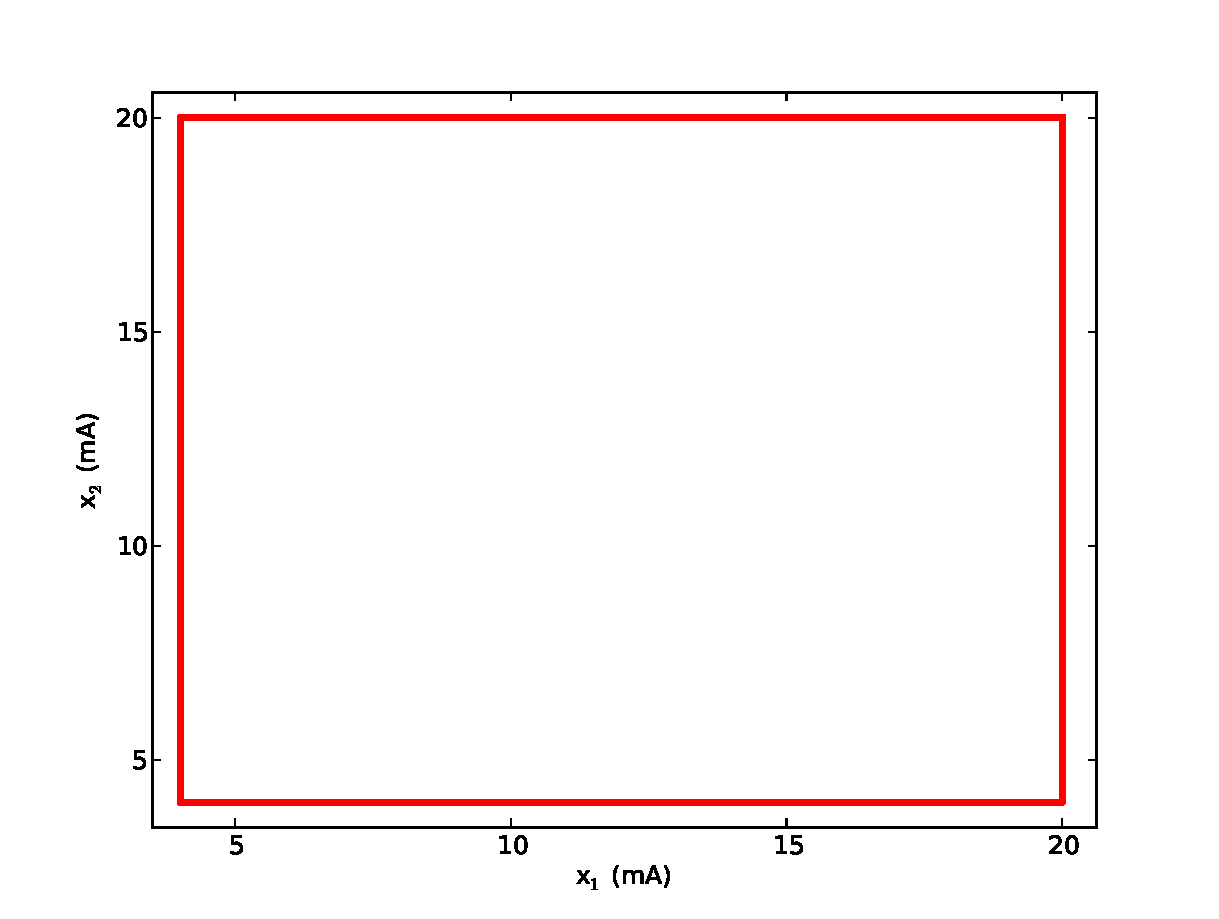
\includegraphics[width=7.8cm]{graph/flowais.pdf}
    \scalebox{1}{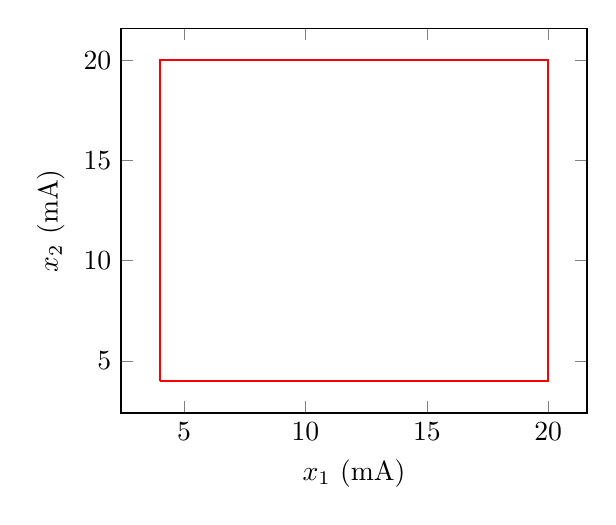
\begin{tikzpicture}
  \begin{axis}[
    width=7.5cm,
    xlabel=$x_1$~(mA),
    ylabel=$x_2$~(mA)]
    \addplot[color=red,thick] coordinates {
      (4,4)
      (4,20)
      (20,20)
      (20,4)
      (4,4)
    };
  \end{axis}
\end{tikzpicture}
}  
    %\qquad
%    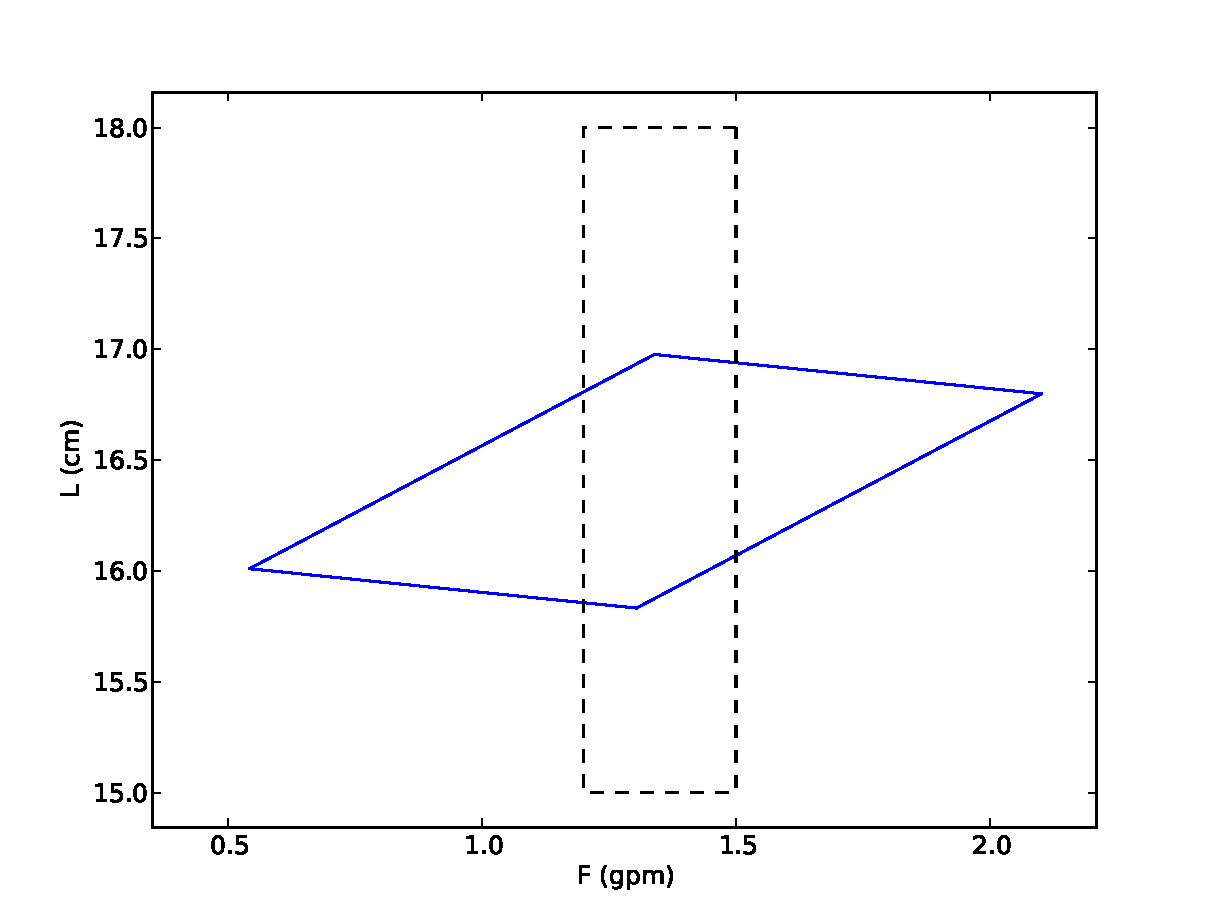
\includegraphics[width=7.8cm]{graph/flowaos.pdf}
    \scalebox{1}{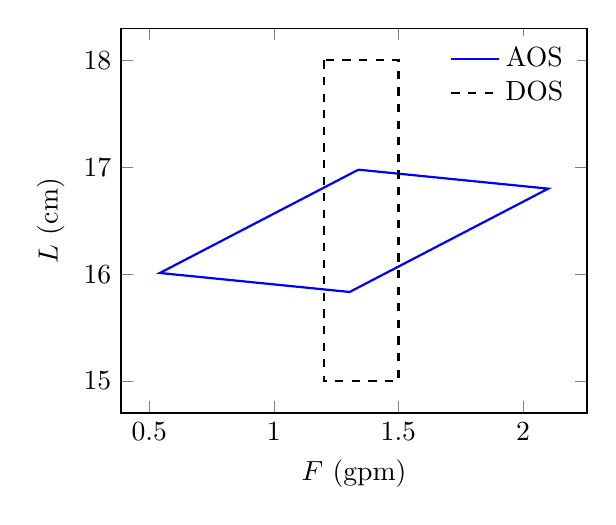
\begin{tikzpicture}
  \begin{axis}[
    width=7.5cm,
    xlabel=$F$~(gpm),
    ylabel=$L$~(cm),
    legend style={
      draw=none}]

    %AOS
    \addplot[color=blue,thick] coordinates {
      (1.3396,  16.9768)
      (2.1012,  16.7992)
      (1.3044,  15.8328)
      (0.5428,  16.0104)
      (1.3396,  16.9768)
    };
    %DOS
    \addplot[color=black,thick,dashed] coordinates {
      (1.2,  18)
      (1.2,  15)
      (1.5,  15)
      (1.5,  18)
      (1.2,  18)
    };
    \legend{AOS,DOS}
  \end{axis}
\end{tikzpicture}
}  
  \caption[AIS, AOS and DOS of the level and flow rig]{AIS (left), AOS and DOS (right) for the level and flow rig.}
  \label{fig:flowaisaos}
\end{figure}

\subsubsection{Set fitting}
It is clear that the level range expectations of this process is too ambitious.
Decreasing these limits will not affect the control adversely, as the model suggests that these upper and lower level limits are not attainable.
Figure~\ref{fig:flowfitbox} shows the fitting of upper and lower operational constraints within the intersection of the AOS and the DOS.
The dark box represents the largest operating region (described only by high and low limits on the outputs) which are within the original DOS and the AOS.
Compared to the DOS as operational constraints, this procedure increases the OI to 1 and presents tighter bounds that are all feasible.

\begin{figure}[htbp]
  \centering
%    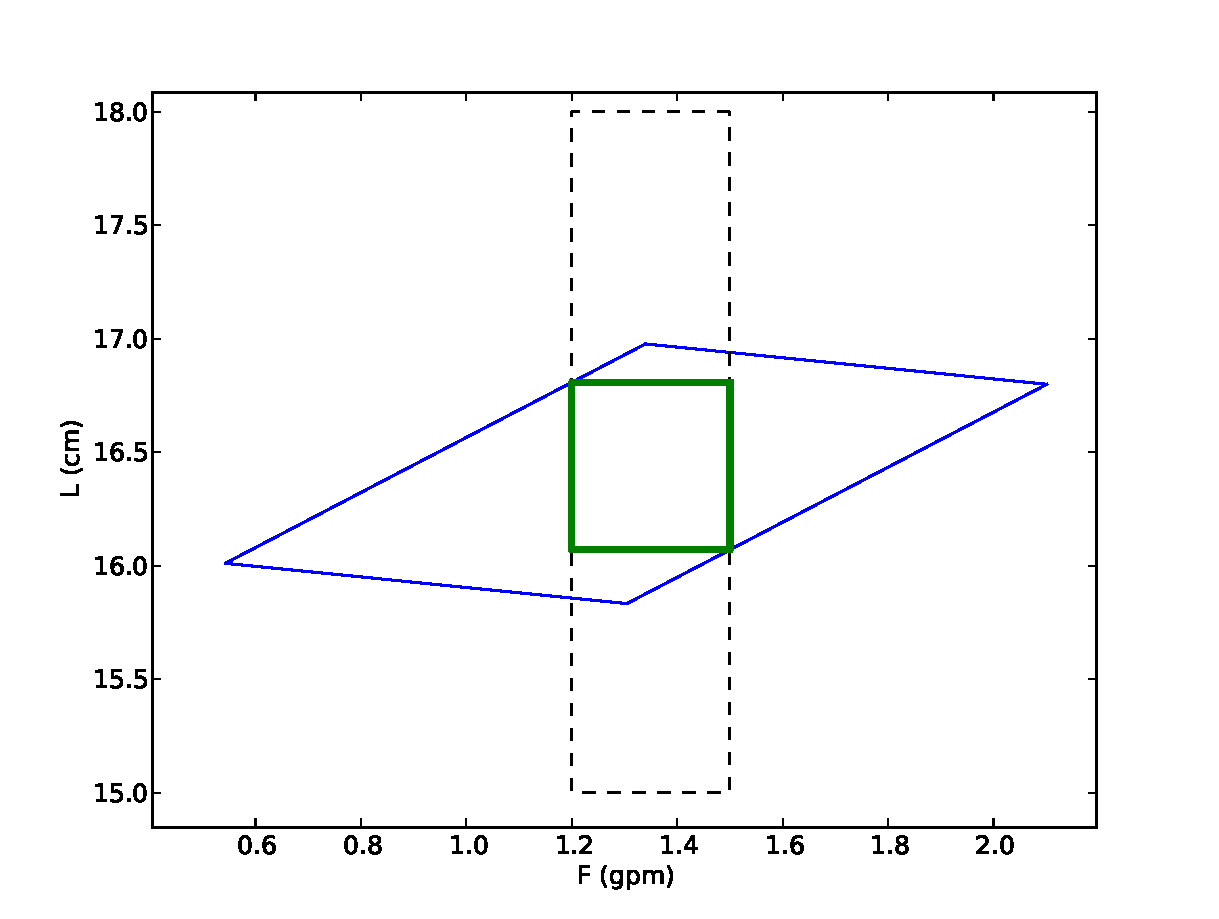
\includegraphics[width=\fullwidth]{graph/flowfitbox.pdf}
    \scalebox{1}{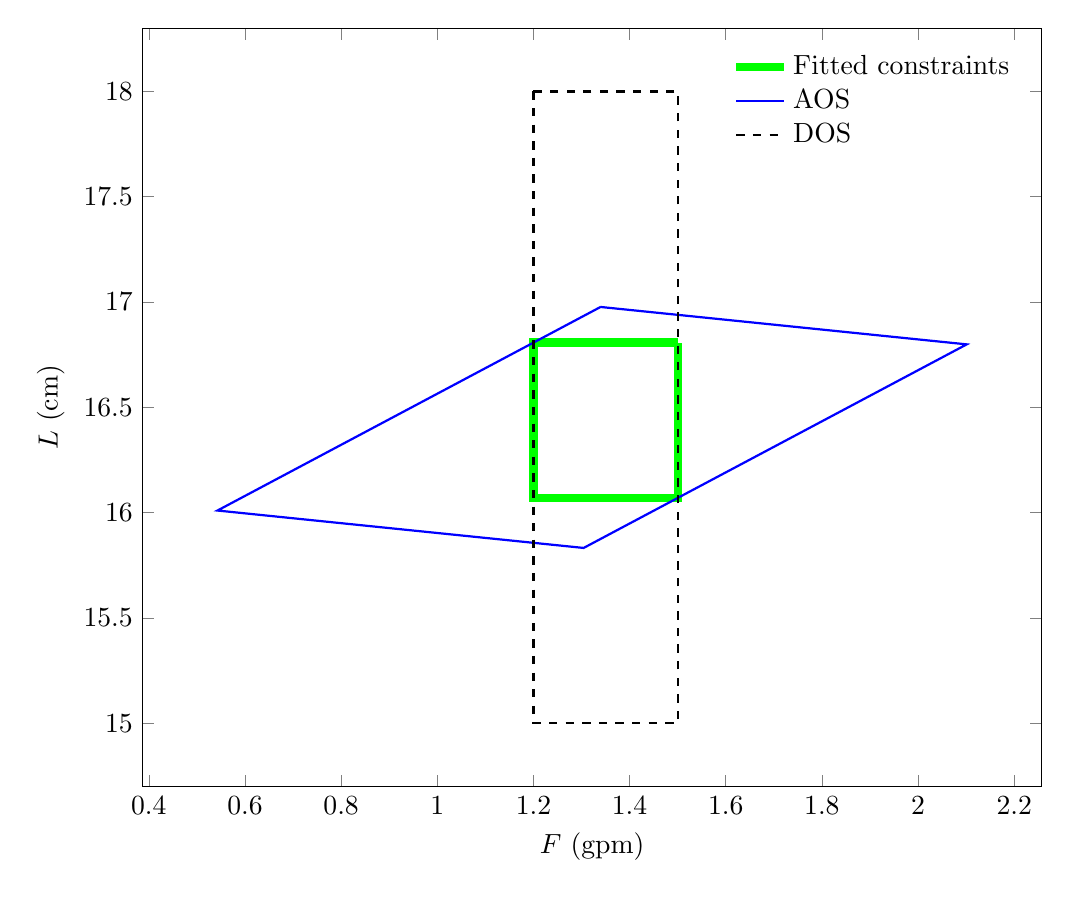
\begin{tikzpicture}
  \begin{axis}[
    width=13cm,
    xlabel=$F$~(gpm),
    ylabel=$L$~(cm),
    legend style={
      cells={anchor=west},
      draw=none}]

    %fitted box
    \addplot[color=green,line width=3pt] coordinates {
      (1.50000041,  16.80748374)
      (1.19999992,  16.80748374)
      (1.19999992,  16.07003455)
      (1.50000041,  16.07003455)
      (1.50000041,  16.80748374)
    };
    %AOS
    \addplot[color=blue,thick] coordinates {
      (1.3396,  16.9768)
      (2.1012,  16.7992)
      (1.3044,  15.8328)
      (0.5428,  16.0104)
      (1.3396,  16.9768)
    };
    %DOS
    \addplot[color=black,thick,dashed] coordinates {
      (1.2,  18)
      (1.2,  15)
      (1.5,  15)
      (1.5,  18)
      (1.2,  18)
    };
    \legend{Fitted constraints,AOS,DOS}
  \end{axis}
\end{tikzpicture}
}  
  \caption{Fitted high and low constraints in the AOS and DOS intersection.}
  \label{fig:flowfitbox}
\end{figure}

\subsubsection{Constraint changes}
As an example of constraint tightening, the newly fitted upper and lower operational constraints of figure~\ref{fig:flowfitbox} is considered and the effect of this constraint change in the input space investigated.
Figure~\ref{fig:flowconsinput} shows the original AIS and DIS, along with the new DIS (the dark dashed box) that corresponds to the changed constraints.
To quantify the tightening of the inputs, the proposed equation~\ref{eq:inputclamp} is used.
This indicates that the attainable movement on the inputs has effectively been tightened by 27\%. 

\begin{figure}[htbp]
  \centering
%    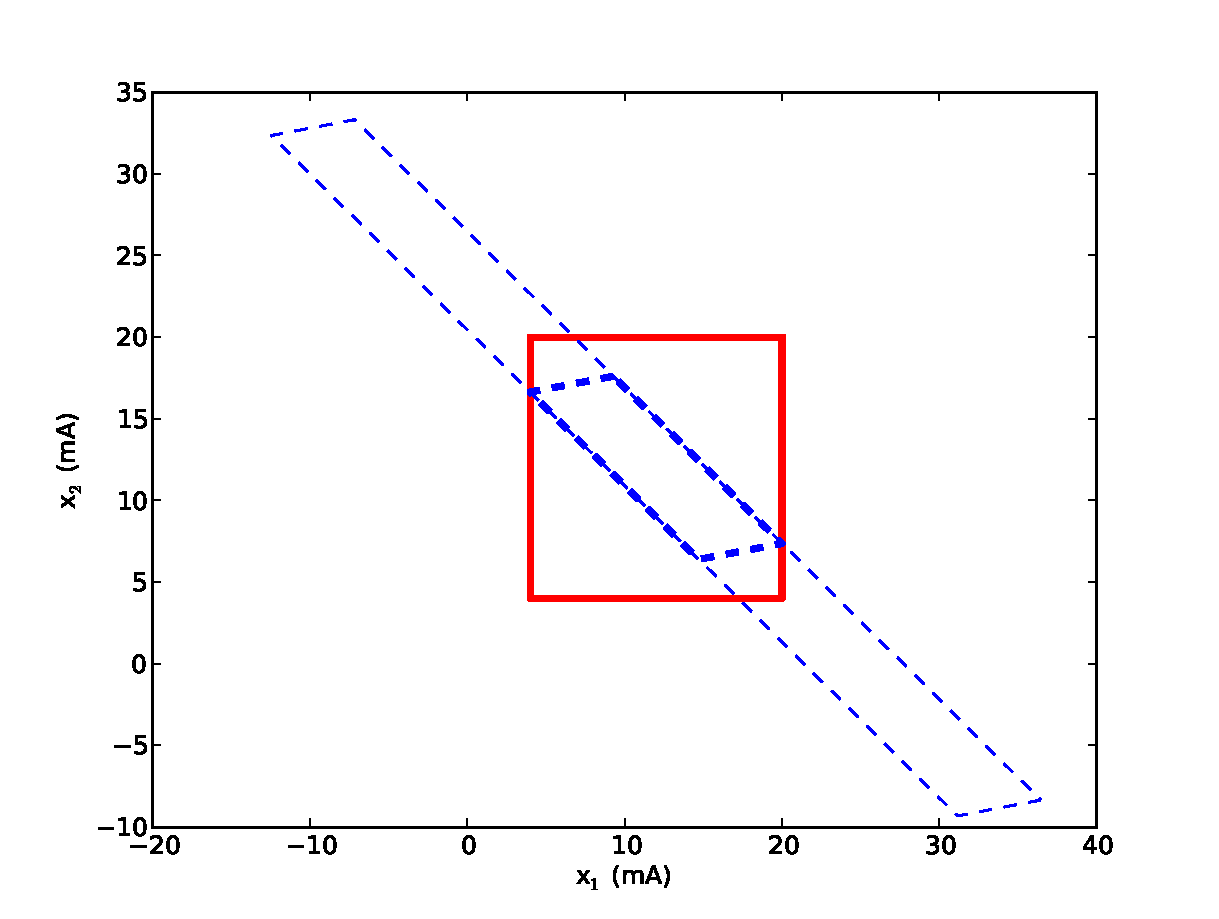
\includegraphics[width=\fullwidth]{graph/flowconsinput.pdf}
    \scalebox{1}{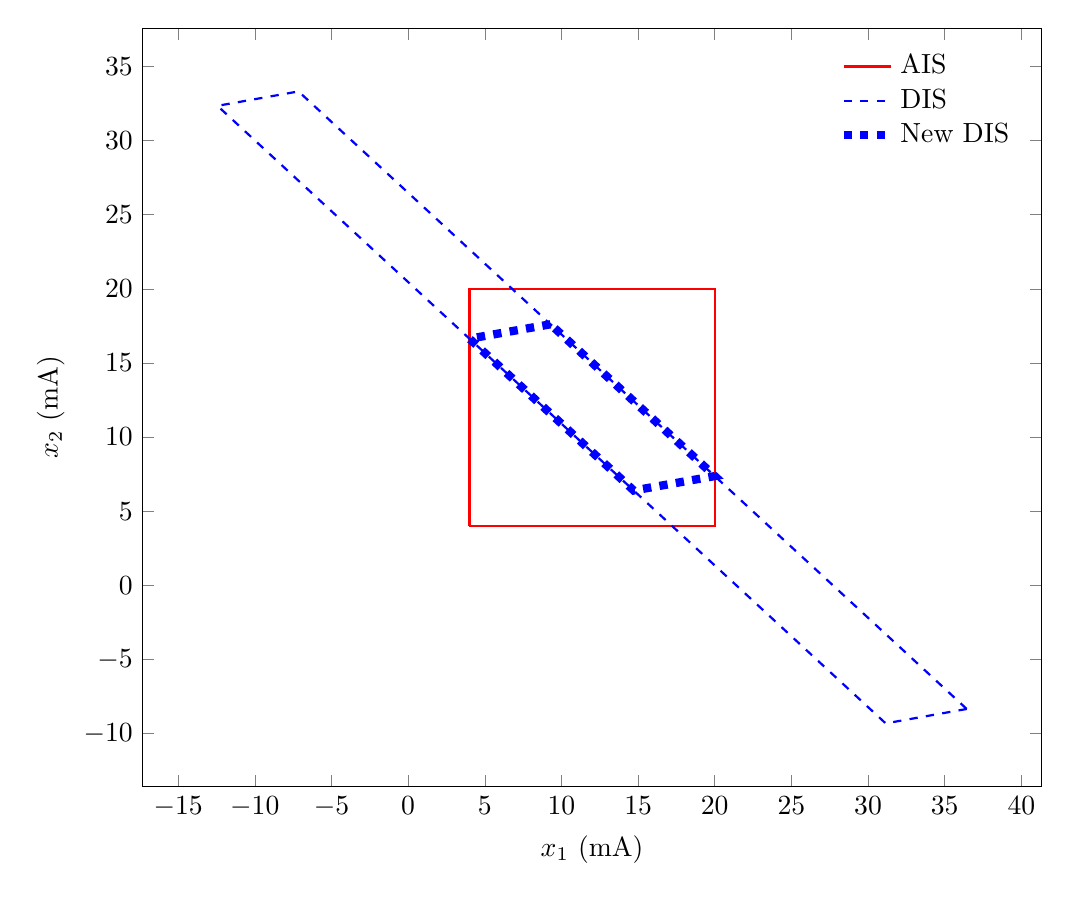
\begin{tikzpicture}
  \begin{axis}[
    width=13cm,
    xlabel=$x_1$~(mA),
    ylabel=$x_2$~(mA),
    legend style={
      cells={anchor=west},
      draw=none}]
    %AIS
    \addplot[color=red,thick] coordinates {
      (4,4)
      (4,20)
      (20,20)
      (20,4)
      (4,4)
    };
    %DIS
    \addplot[color=blue,thick,dashed] coordinates {
      (36.43535542,  -8.34383369)
      (31.14919687,  -9.3152966 )
      (-12.43535542,  32.34383369)
      (-7.14919687,  33.3152966)
      (36.43535542,  -8.34383369)
    };
    %DISn
    \addplot[color=blue,line width=3pt,dashed] coordinates {
      (9.28618489,  17.6059809)
      (4.00001755,  16.63451637)
      (14.71381511,   6.3940191)
      (19.99998245,   7.36548363)
      (9.28618489,  17.6059809)
    };
    \legend{AIS,DIS,New DIS}
  \end{axis}
\end{tikzpicture}
}  
  \caption[AIS, DIS and newly fitted DIS of level and flow rig]{Newly fitted constraint set shows feasible input constraints as opposed to those of the original DOS.}
  \label{fig:flowconsinput}
\end{figure}

The unattainable limits of the DOS are just as clear in the input space (DIS).
This figure also serves to confirm that the newly fitted constraints on the outputs correspond to a fully attainable region in the input space.

\subsubsection{Constraint types}
As mentioned in section~\ref{sec:commercialmpc}, the only constraint validation done by both RMPCT and DMCplus is checking whether the operational constraints are within the engineering constraints.
Figure~\ref{fig:flowcontypes} shows the AOS and the physical constraints of the system (which are typically used to specify the engineering constraints).
It is clear that with only checking against physical constraints (and disregarding the system model), specification of operational constraints that are completely unattainable is possible.

Figure~\ref{fig:flowcontypes} also shows the fitting of a revised set of engineering limits with a safety factor of 20\%.
This new set of engineering limits represents the attainable region of the process as well as the physical constraints of the system.
The risk of specifying operational constraints that are not attainable has also been reduced.

\begin{figure}[htbp]
  \centering
%    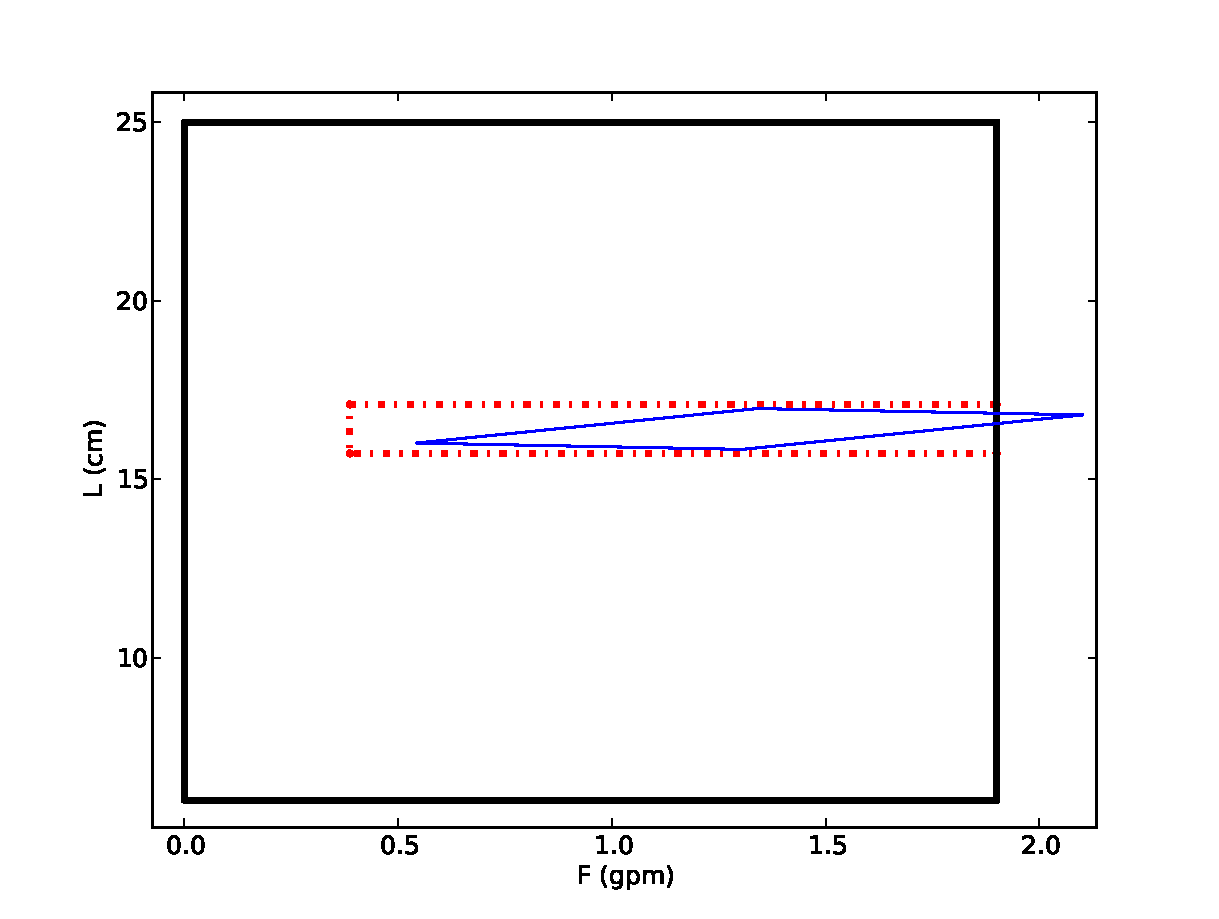
\includegraphics[width=\fullwidth]{graph/flowcontypes.pdf}
    \scalebox{1}{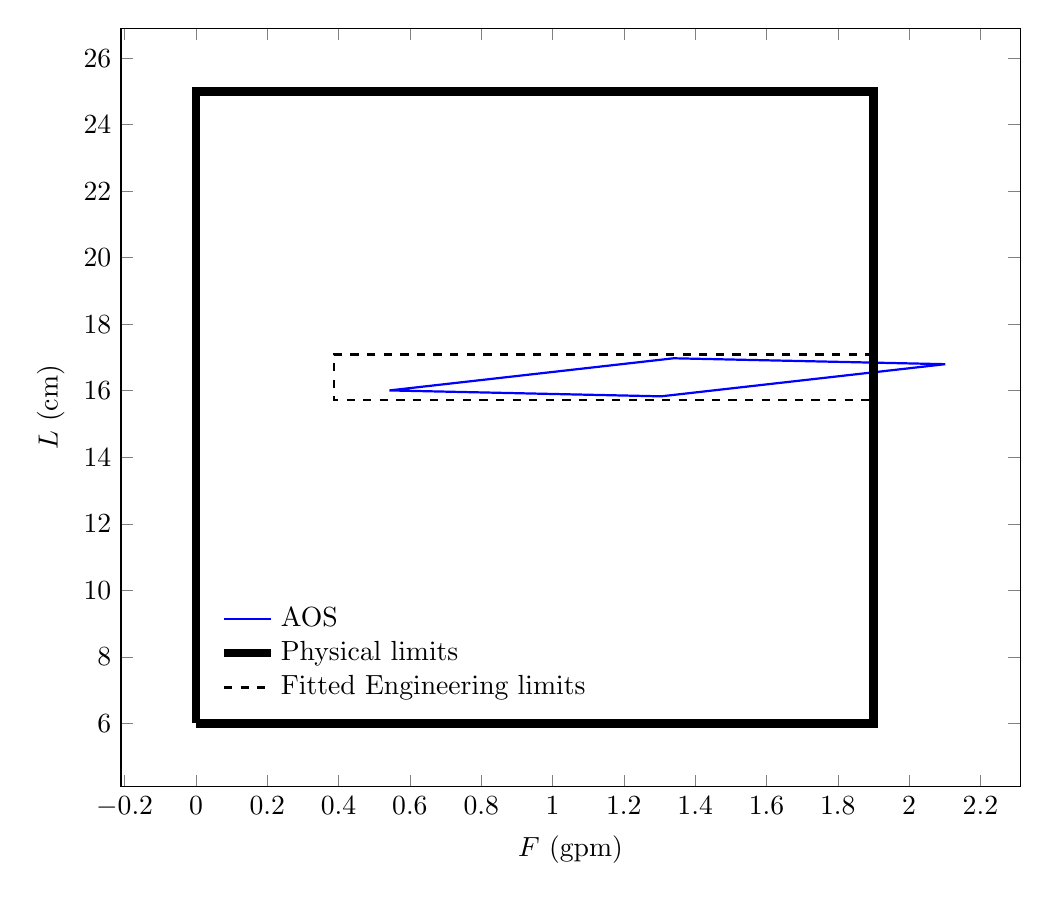
\begin{tikzpicture}
  \begin{axis}[
    width=13cm,
    xlabel=$F$~(gpm),
    ylabel=$L$~(cm),
    legend style={
      cells={anchor=west},
      at={(0.1,0.1)},
      anchor=south west,
      draw=none}]

    %AOS
    \addplot[color=blue,thick] coordinates {
      (1.3396,  16.9768)
      (2.1012,  16.7992)
      (1.3044,  15.8328)
      (0.5428,  16.0104)
      (1.3396,  16.9768)
    };
    %Physical limits
    \addplot[color=black,line width=3pt] coordinates {
      (0,  6)
      (0,  25)
      (1.9, 25)
      (1.9, 6)
      (0,  6)
    };
    %Fitted Eng limits
    \addplot[color=black,thick,dashed] coordinates {
      (1.9,      17.0912)
      (0.38696,  17.0912)
      (0.38696,  15.7184)
      (1.9,      15.7184)
      (1.9,      17.0912)
    };
    \legend{AOS,Physical limits,Fitted Engineering limits}
  \end{axis}
\end{tikzpicture}
}  
  \caption[Physical constraint region of level and flow rig]{Physical constraint region, AOS and revised engineering limits (with a 20\% safety factor) for the level and flow rig.}
  \label{fig:flowcontypes}
\end{figure}


\subsection{Laboratory distillation column}
\subsubsection{Input and Output spaces}
From the data in table~\ref{tab:columnopcon} and equation~\ref{eq:columnmodel} the AIS and AOS of the laboratory distillation column can be generated as shown in figure~\ref{fig:columnaisaos}.
The operating constraints for $R$ are used to construct the AIS as values outside of this range (although possible) cause the validity of the linear model to diminish.
The DOS, as described by the operating range in table~\ref{tab:columnopcon}, is also shown.

\begin{figure}[htbp]
  \centering
%    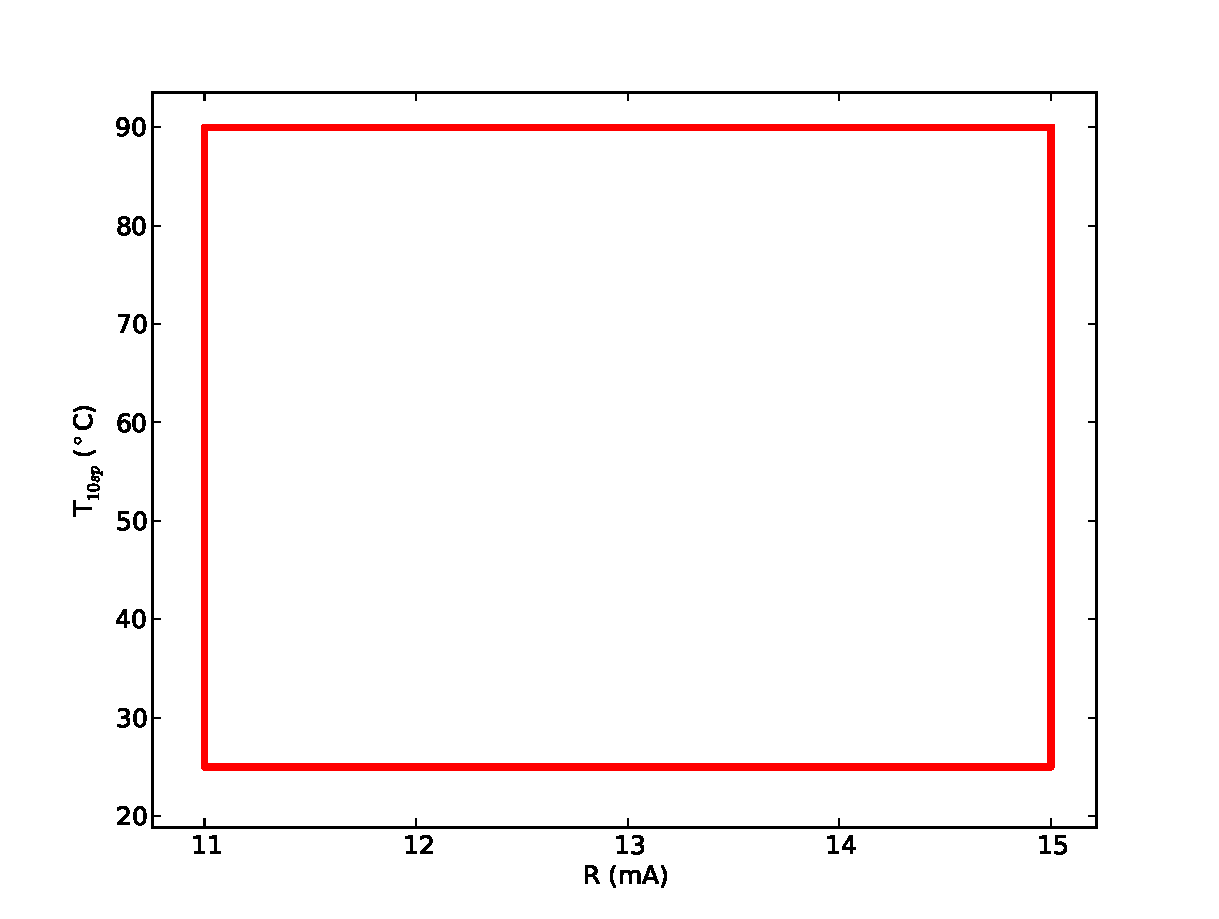
\includegraphics[width=7.8cm]{graph/columnais.pdf}
    \scalebox{1}{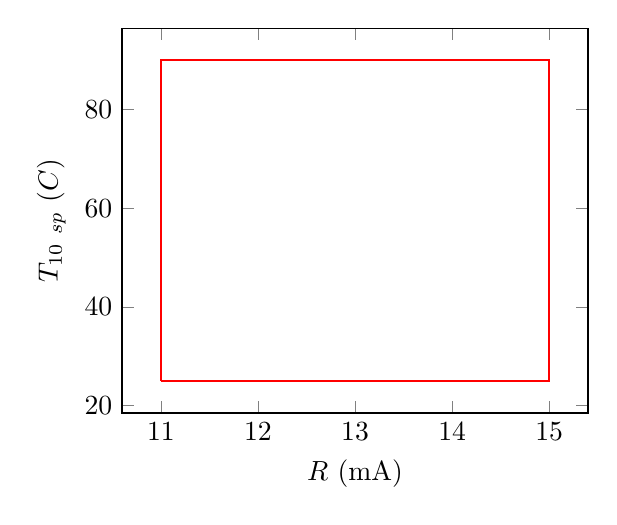
\begin{tikzpicture}
  \begin{axis}[
    width=7.5cm,
    xlabel=$R$~(mA),
    ylabel=$T_{10~sp}$~($\degrees{C}$)]
    \addplot[color=red,thick] coordinates {
      (11,25)
      (11,90)
      (15,90)
      (15,25)
      (11,25)
    };
  \end{axis}
\end{tikzpicture}
}  
    %\qquad
%    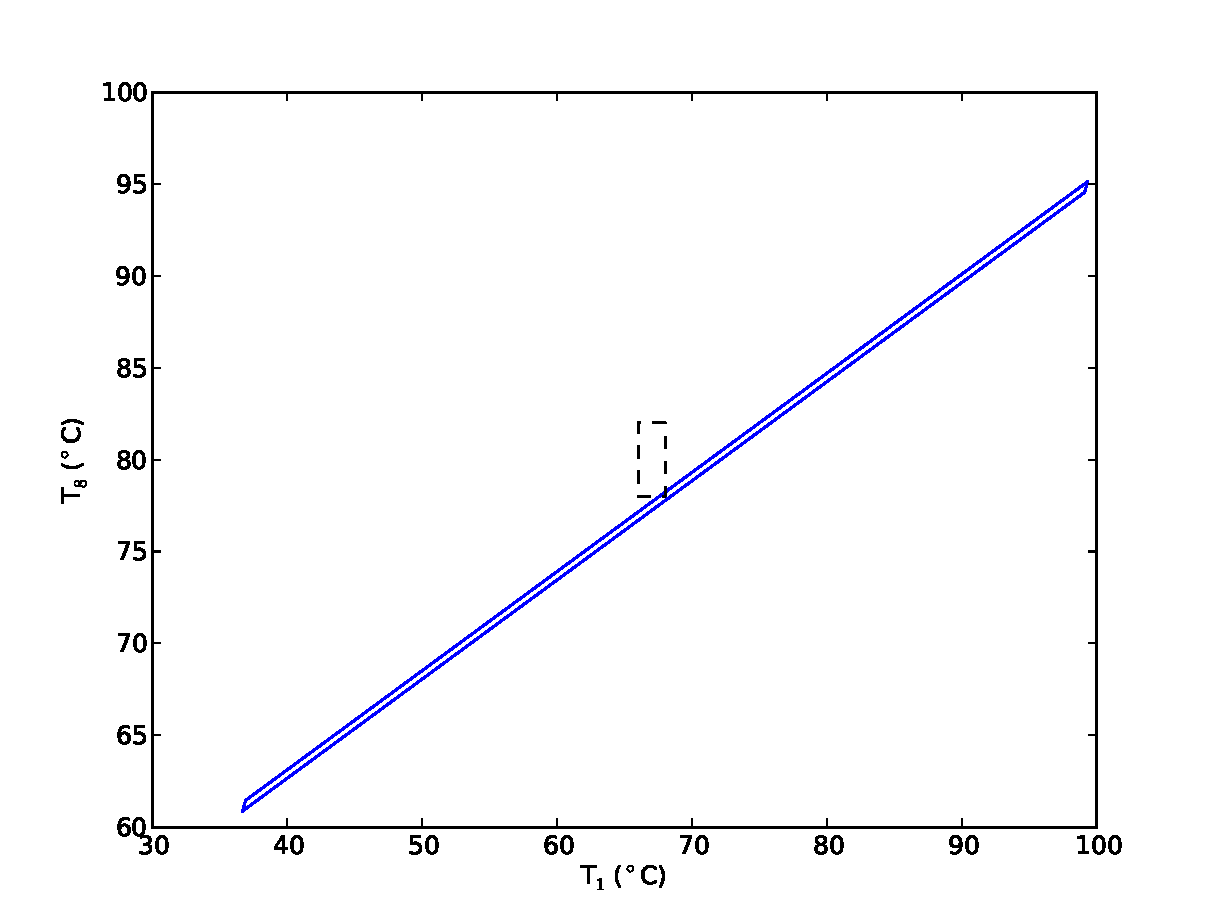
\includegraphics[width=7.8cm]{graph/columnaos.pdf}
    \scalebox{1}{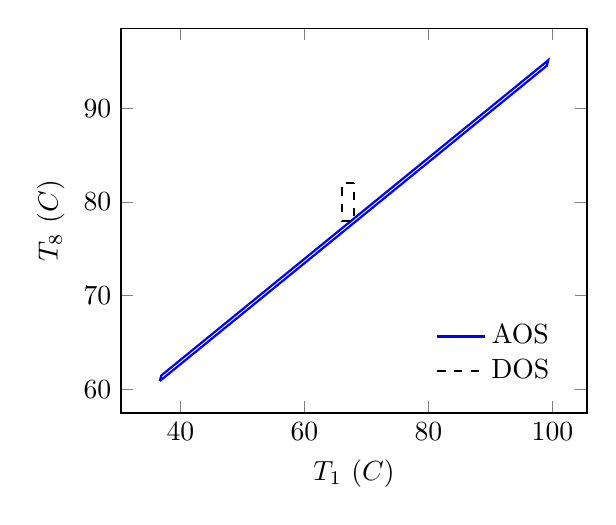
\begin{tikzpicture}
  \begin{axis}[
    width=7.5cm,
    xlabel=$T_1$~($\degrees{C}$),
    ylabel=$T_8$~($\degrees{C}$),
    legend style={
      draw=none,
      at={(0.95,0.05)},
      anchor=south east}]

    %AOS
    \addplot[color=blue,thick] coordinates {
      (36.685,  60.873) 
      (36.915,  61.457) 
      (99.315,  95.127) 
      (99.085,  94.543) 
      (36.685,  60.873) 
    };
    %DOS
    \addplot[color=black,thick,dashed] coordinates {
      (68.,  82.)
      (66.,  82.)
      (66.,  78.)
      (68.,  78.)
      (68.,  82.)
    };
    \legend{AOS,DOS}
  \end{axis}
\end{tikzpicture}
}  
  \caption[AIS, AOS and DOS of the laboratory distillation column]{AIS (left), AOS and DOS (right) of the laboratory distillation column.}
  \label{fig:columnaisaos}
\end{figure}

Figure~\ref{fig:columnaosfocus} focuses on the intersection of the AOS and the DOS.
The calculated OI is 0.006 which confirms that only a very small operating region within the DOS is attainable.
It is also clear that the upper limit of 82$\degrees{C}$ on $T_8$ is unrealistic as the maximum value of $T_8$ (in the operating region) is only 78.2$\degrees{C}$.

\begin{figure}[htbp]
  \centering
%    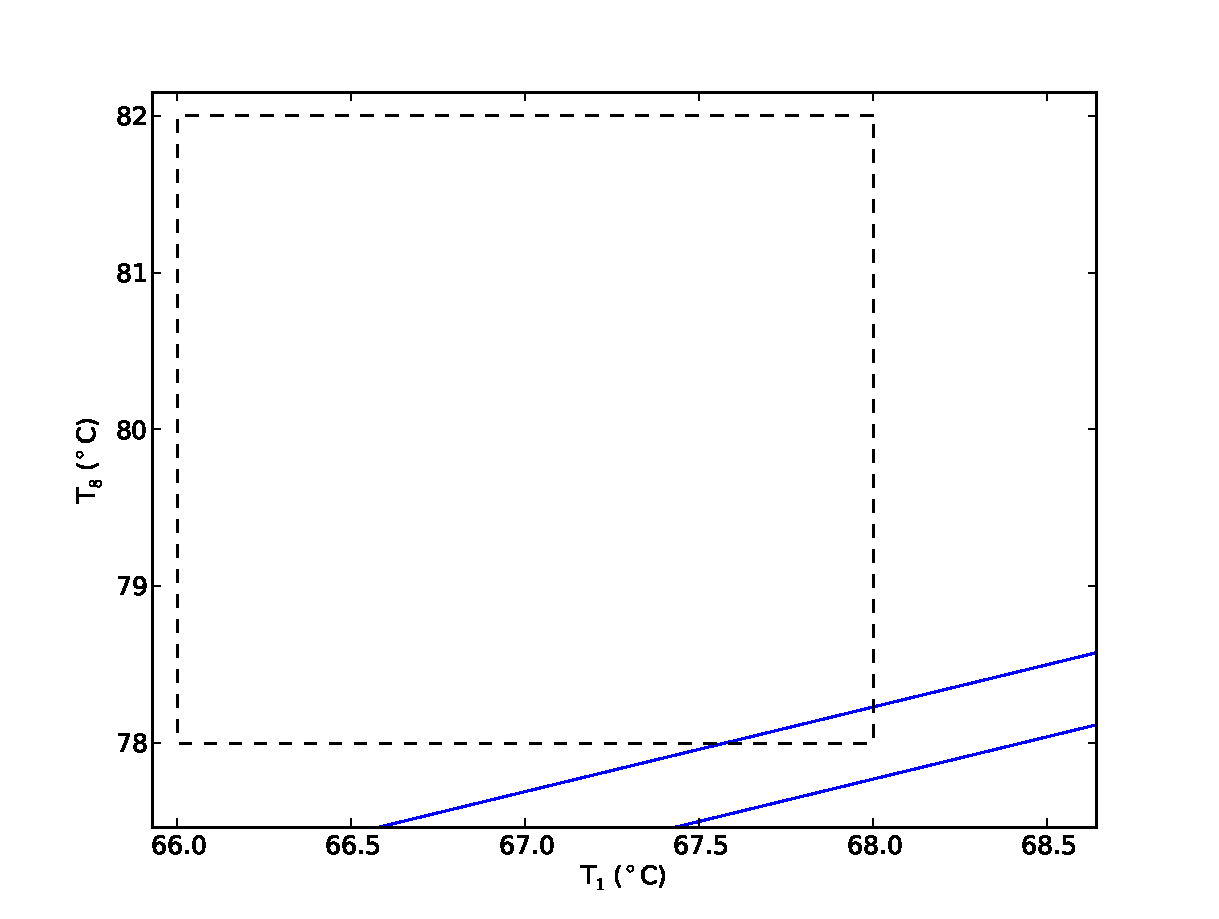
\includegraphics[width=\fullwidth]{graph/columnaosfocus.pdf}
    \scalebox{1}{\begin{tikzpicture}
  \begin{axis}[
    width=13cm,
    xlabel=$T_1$~($\degrees{C}$),
    ylabel=$T_8$~($\degrees{C}$),
    xmin=65.8,xmax=68.7,ymin=77.8,ymax=82.2,
    xtick={66,66.5,...,68.5},
    ytick={78,78.5,...,82},
    legend style={
      draw=none}]

    %AOS
    \addplot[color=blue,thick] coordinates {
      (36.685,  60.873) 
      (36.915,  61.457) 
      (99.315,  95.127) 
      (99.085,  94.543) 
      (36.685,  60.873) 
    };
    %DOS
    \addplot[color=black,thick,dashed] coordinates {
      (68.,  82.)
      (66.,  82.)
      (66.,  78.)
      (68.,  78.)
      (68.,  82.)
    };
    \legend{AOS,DOS}
  \end{axis}
\end{tikzpicture}
}  
  \caption[AOS and DOS intersection of the laboratory distillation column]{The AOS and DOS intersection shows a very small operating region.}
  \label{fig:columnaosfocus}
\end{figure}

\subsubsection{Set fitting}
Figure~\ref{fig:columnfitbox} focuses even closer on the AOS and DOS intersection.
The constraints representing the intersection (dark triangle) and a fitted set of high and low limits (dark dashed box) are also shown.
The fitted limits within the intersection shows that the operating region is essentially an operating point with temperatures only having a span of about 0.1$\degrees{C}$.
In practice the DOS would be adjusted or the model re-evaluated, but for the sake of illustrating the outputs of the method, the DOS will be kept as is.
  
\begin{figure}[htbp]
  \centering
%    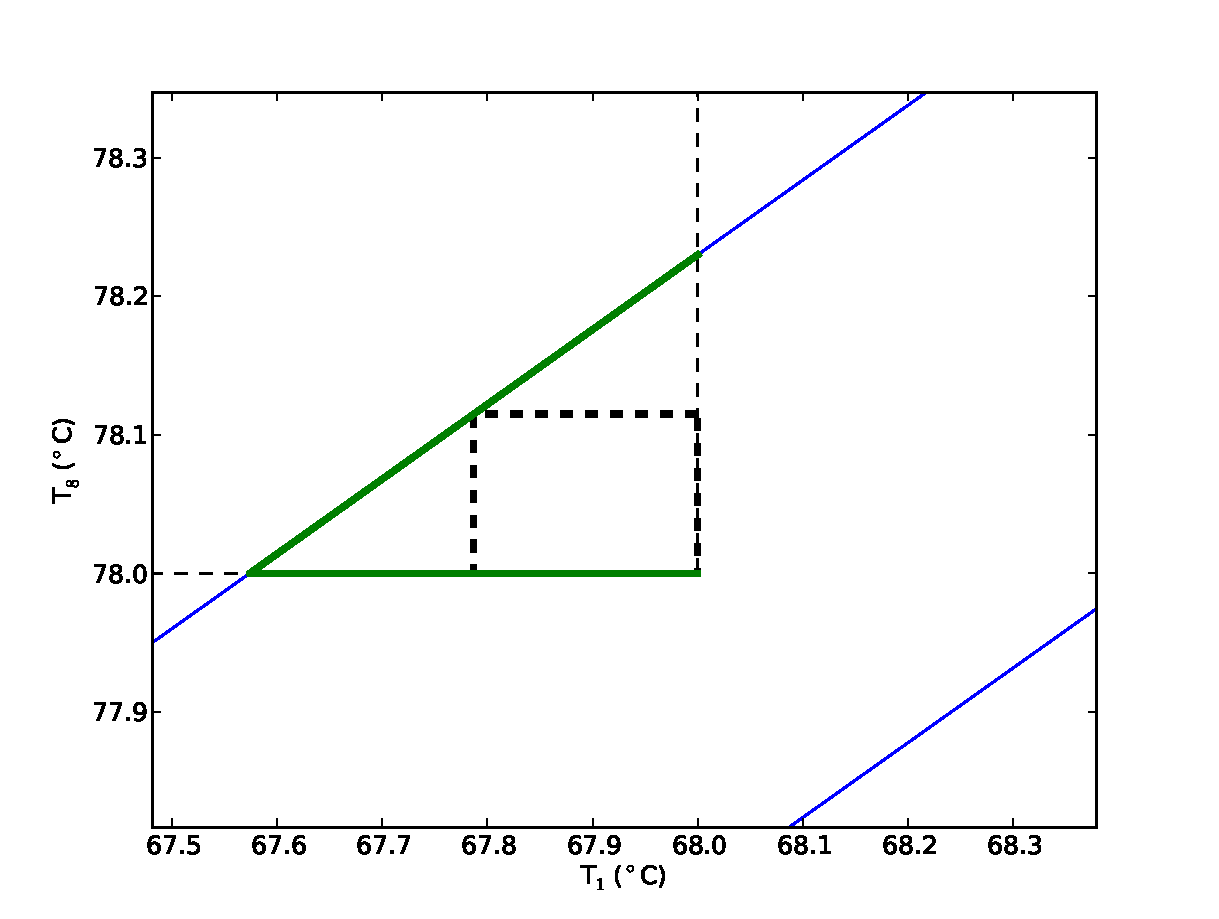
\includegraphics[width=\fullwidth]{graph/columnfitbox.pdf}
    \scalebox{1}{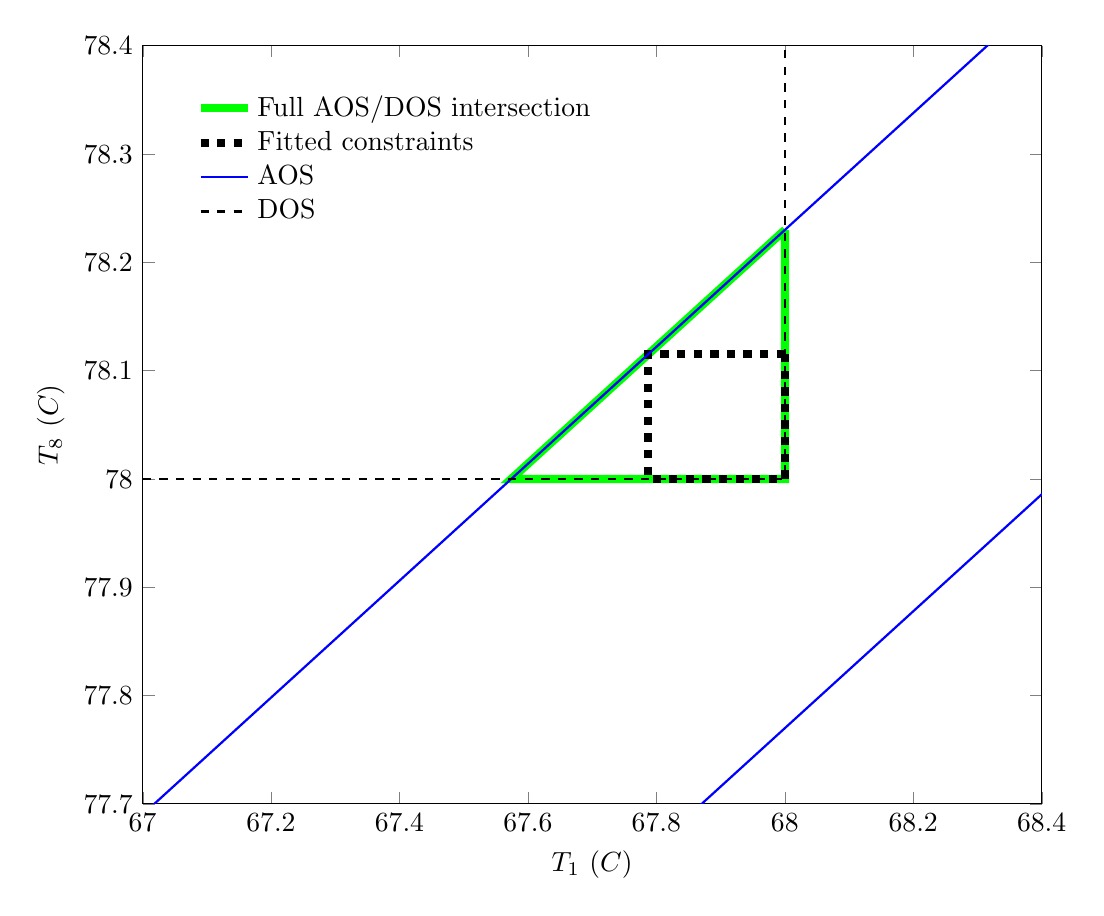
\begin{tikzpicture}
  \begin{axis}[
    width=13cm,
    xlabel=$T_1$~($\degrees{C}$),
    ylabel=$T_8$~($\degrees{C}$),
    xmin=67,xmax=68.4,ymin=77.7,ymax=78.4,
    xtick={67,67.2,...,68.4},
    ytick={77.7,77.8,...,78.4},
    legend style={
      draw=none,
      at={(0.05,0.95)},
      anchor=north west,
      cells={anchor=west}}]

    %intersection
    \addplot[color=green,line width=3pt] coordinates {
      (68.      ,   78.2299483)
      (67.573841,   78.       )
      (68.      ,   78.       )
      (68.      ,   78.2299483)
    };
    %fitted cons
    \addplot[color=black,line width=3pt,dashed] coordinates {
      (67.99999975,  78.11504787)
      (67.78705642,  78.11504787)
      (67.78705642,  77.99999994)
      (67.99999975,  77.99999994)
      (67.99999975,  78.11504787)
    };
   %AOS
    \addplot[color=blue,thick] coordinates {
      (36.685,  60.873) 
      (36.915,  61.457) 
      (99.315,  95.127) 
      (99.085,  94.543) 
      (36.685,  60.873) 
    };
    %DOS
    \addplot[color=black,thick,dashed] coordinates {
      (68,  82)
      (66,  82)
      (66,  78)
      (68,  78)
      (68,  82)
    };
     \legend{Full AOS/DOS intersection,Fitted constraints,AOS,DOS}
  \end{axis}
\end{tikzpicture}
}  
  \caption[Fitted constraints for the laboratory distillation column]{Intersection of AOS and DOS with fitted high and low limits for the column tray temperatures.}
  \label{fig:columnfitbox}
\end{figure}

If constraints specifying the full intersection in figure~\ref{fig:columnfitbox} is used as operational constraints, an additional variable needs to be added to the system (along with its associated high and low limits).
Using the fitted box constraints as operational constraints only require the high and low limits of the existing variables to be changed.
The full intersection does, however, have the advantage of a 200\% larger operating region at the cost of a larger control problem.

\subsubsection{Constraint reformatting}
To use the constraints describing the whole intersection in figure~\ref{fig:columnfitbox}, the set needs to be reformatted to be compatible with commercial MPC packages, as they only accept high and low limits.

An additional variable needs to be added to the process model and the diagonal constraint ($0.88T_8-0.47T_1\leq 36.56\degrees{C} $) needs to be expressed as a high and low limit on this variable.

Naming the new output $y_3$ and augmenting the process model matrix as per equation~\ref{eq:linconoutput} results in equation~\ref{eq:columnnewmodel}.
The diagonal (linear) constraint can now be expressed as {$y_3~\leq~36.56\degrees{C}$}.

\begin{equation}
  \label{eq:columnnewmodel}
  G_{col-new}= \bpm -0.0575 & 0.96 \\       % T1
                  -0.146  & 0.518 \\      % T8
                   0.0956 & 1.30 \\ \epm  %   y3
\end{equation}

\subsection{MPC interfacing}
The operator interfaces for RMPCT and DMCplus will be used to enter the operational constraints determined from the method.
For RMPCT (figure~\ref{fig:ssrmpctoperator}) the shaded columns labeled ``Low Limit'' and ``High Limit'' are used.
For DMCplus (figure~\ref{fig:ssdmcplusoperator}) the column labeled ``Lower Limit'' and ``Upper Limit'' are used.

The revised engineering limits for the level and flow rig would be added to the controller via the building interfaces (figures~\ref{fig:ssrmpctcontrolbuild} and \ref{fig:ssdmcpluscontrolbuild}).

The modelling interfaces (figures~\ref{fig:ssrmpctmodel} and \ref{fig:ssdmcplusmodel}) are used to augment the model for the addition of unmeasured variables, as determined for the distillation column.

\section{Constraint set fitting}
The fitting of constraint sets, which form a large part of this dissertation, is discussed separately.
Observations made while studying the fitting of constraint sets, which could lead to future research is discussed in section~\ref{sec:setfitfuture}.

\subsection{Solution times}
The use of constrained, gradient-based solvers proved to be significantly faster than unconstrained solvers.
Inconsistent gradient information does, however, hamper their implementation.

Figure~\ref{fig:cubefittime} compares the solution times of the constrained, gradient based solver (henceforth referred to as SLSQP) and the unconstrained solver (henceforth referred to as simplex) for rectangular set fitting.
Arbitrary sets with three constraints on two variables were generated.
A high and low constraint set was fitted within the attainable region of the initial three constraints.
The data in figure~\ref{fig:cubefittime} is expressed as the fraction of tests that completed successfully within the given number of function evaluations.

\begin{figure}[htbp]
  \centering
%    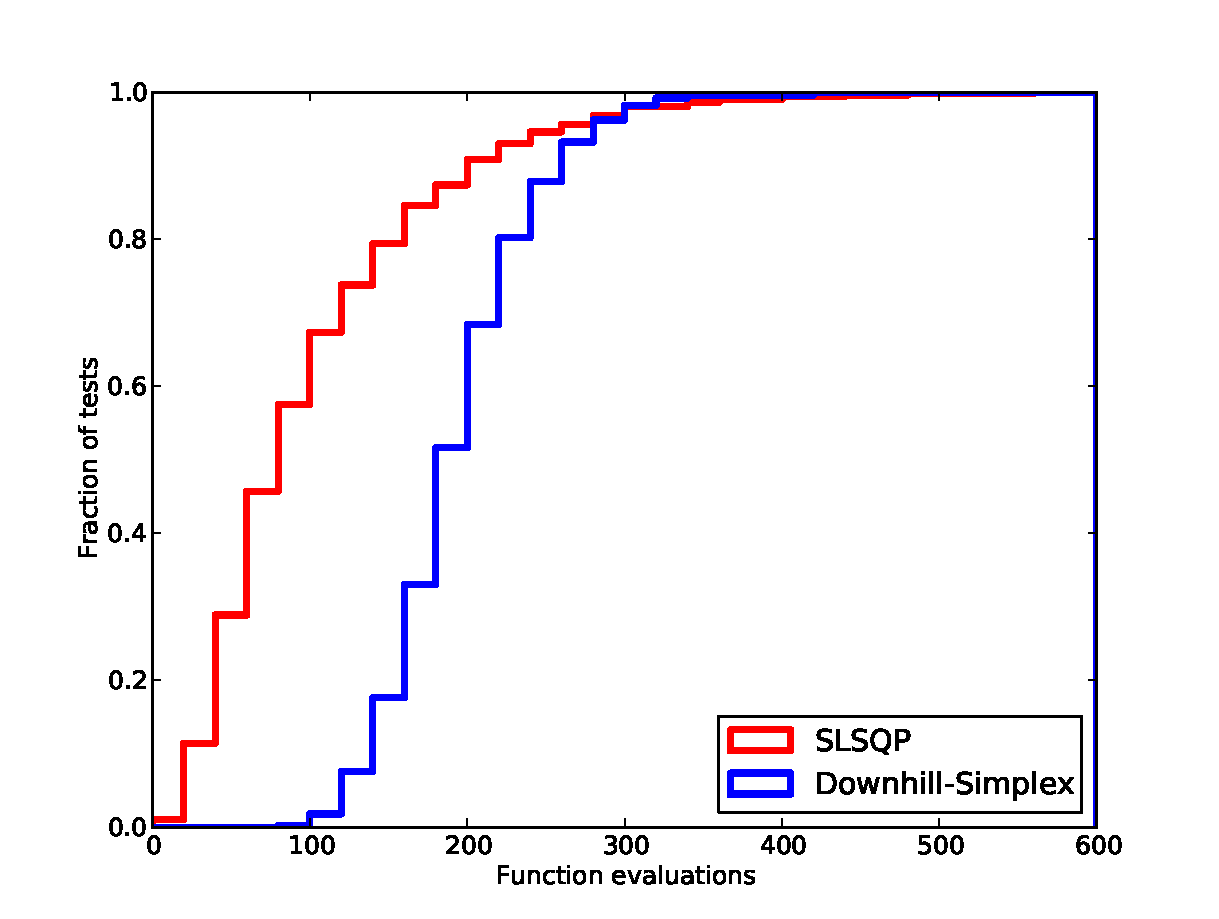
\includegraphics[width=\fullwidth]{graph/cubefittime}
    \scalebox{1}{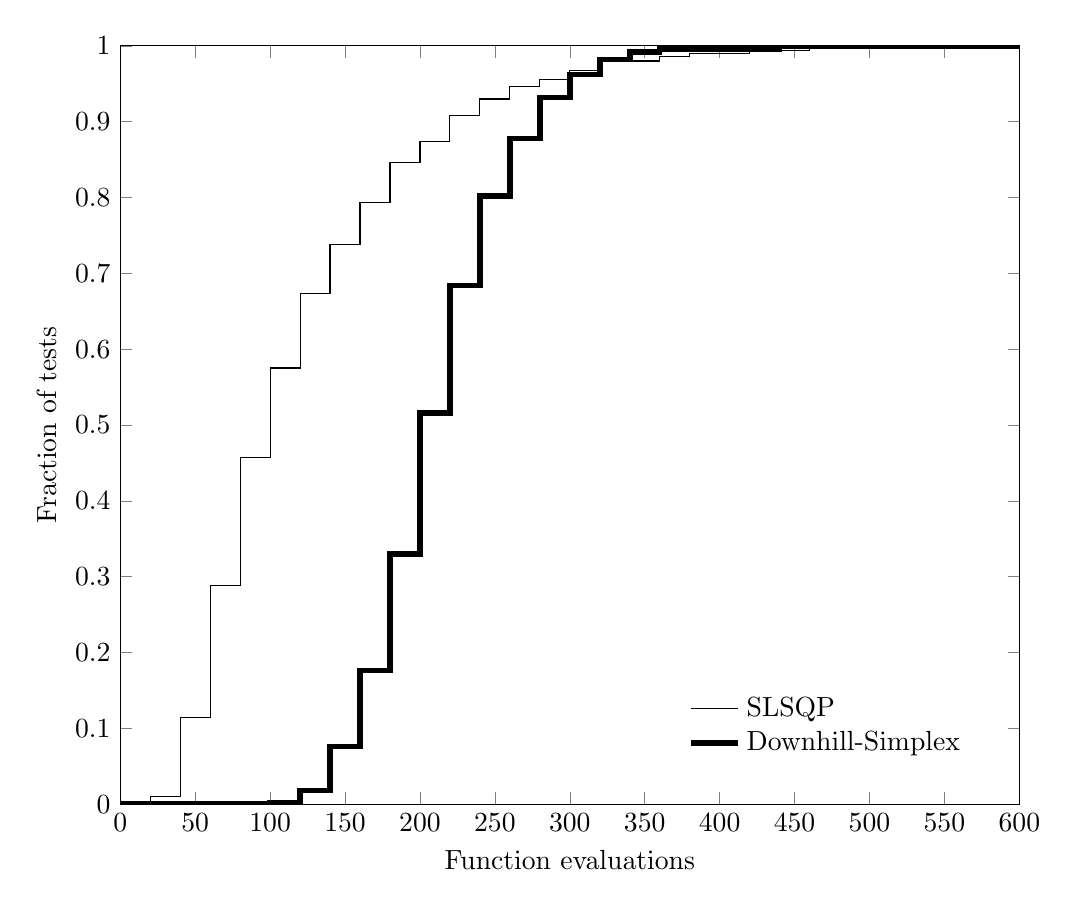
\begin{tikzpicture}
  \begin{axis}[
    width=13cm,
    ylabel=Fraction of tests,
    xlabel=Function evaluations,
    xmin=0,xmax=600,ymin=0,ymax=1,
    legend style={
      draw=none,
      at={(0.95,0.05)},
      anchor=south east,
      cells={anchor=west}}]
    \addplot [const plot] coordinates {
(0.00000000e+00, 0.00000000e+00)
(2.00000000e+01, 1.00200401e-02)
(4.00000000e+01, 1.14228457e-01)
(6.00000000e+01, 2.88577154e-01)
(8.00000000e+01, 4.56913828e-01)
(1.00000000e+02, 5.75150301e-01)
(1.20000000e+02, 6.73346693e-01)
(1.40000000e+02, 7.37474950e-01)
(1.60000000e+02, 7.93587174e-01)
(1.80000000e+02, 8.45691383e-01)
(2.00000000e+02, 8.73747495e-01)
(2.20000000e+02, 9.07815631e-01)
(2.40000000e+02, 9.29859719e-01)
(2.60000000e+02, 9.45891784e-01)
(2.80000000e+02, 9.55911824e-01)
(3.00000000e+02, 9.67935872e-01)
(3.20000000e+02, 9.79959920e-01)
(3.40000000e+02, 9.79959920e-01)
(3.60000000e+02, 9.85971944e-01)
(3.80000000e+02, 9.89979960e-01)
(4.00000000e+02, 9.89979960e-01)
(4.20000000e+02, 9.93987976e-01)
(4.40000000e+02, 9.93987976e-01)
(4.60000000e+02, 9.95991984e-01)
(4.80000000e+02, 9.95991984e-01)
(5.00000000e+02, 9.97995992e-01)
(5.20000000e+02, 9.97995992e-01)
(5.40000000e+02, 9.97995992e-01)
(5.60000000e+02, 9.97995992e-01)
(5.80000000e+02, 1.00000000e+00)
(6.00000000e+02, 1.00000000e+00)
    };
    \addplot [const plot,line width=2pt] coordinates {
(0.00000000e+00, 0.00000000e+00)
(2.00000000e+01, 0.00000000e+00)
(4.00000000e+01, 0.00000000e+00)
(6.00000000e+01, 0.00000000e+00)
(8.00000000e+01, 0.00000000e+00)
(1.00000000e+02, 2.00000000e-03)
(1.20000000e+02, 1.80000000e-02)
(1.40000000e+02, 7.60000000e-02)
(1.60000000e+02, 1.76000000e-01)
(1.80000000e+02, 3.30000000e-01)
(2.00000000e+02, 5.16000000e-01)
(2.20000000e+02, 6.84000000e-01)
(2.40000000e+02, 8.02000000e-01)
(2.60000000e+02, 8.78000000e-01)
(2.80000000e+02, 9.32000000e-01)
(3.00000000e+02, 9.62000000e-01)
(3.20000000e+02, 9.82000000e-01)
(3.40000000e+02, 9.92000000e-01)
(3.60000000e+02, 9.96000000e-01)
(3.80000000e+02, 9.96000000e-01)
(4.00000000e+02, 9.96000000e-01)
(4.20000000e+02, 9.96000000e-01)
(4.40000000e+02, 1.00000000e+00)
(4.60000000e+02, 1.00000000e+00)
(4.80000000e+02, 1.00000000e+00)
(5.00000000e+02, 1.00000000e+00)
(5.20000000e+02, 1.00000000e+00)
(5.40000000e+02, 1.00000000e+00)
(5.60000000e+02, 1.00000000e+00)
(5.80000000e+02, 1.00000000e+00)
(6.00000000e+02, 1.00000000e+00)    };
    \legend{SLSQP,Downhill-Simplex}
  \end{axis}
\end{tikzpicture}
}  
  \caption[SLSQP and simplex calculation time comparison]{Cumulative plot of function evaluations showing faster execution of SLSQP when compared to simplex}
  \label{fig:cubefittime}
\end{figure}

Fitting a constraint set of an arbitrary size was unsuccessful using constrained, gradient-based solvers.
Possible reasons for this is inconsistent gradient information regarding the position of vertices outside the initial set and the superfluous degrees of freedom present in the problem formulation.
The sources of these problems are discussed in the accompanying code manual and program listing.

\subsection{Accuracy}\label{sec:fittingaccuracy}
The solutions for high and low constraint set fitting resulted in an optimal answer for each test.
The fitting of arbitrary sized constraint sets suffered from accuracy issues due to the high dependence on the starting point.
As mentioned in the preceding section, due to problems with the unconstrained, gradient-based solvers, only simplex was used for the fitting of arbitrary sets.

\subsubsection{Two variable systems}\label{sec:2dfitting}
For these tests, a 3-constraint set was fitted into a 4-constraint set.
The initial set was chosen to be rectangular (high and low limits) to enable the algebraic calculation of the optimal fitted set.
The optimal solution is 50\% of the volume (area in 2 dimensions) of the initial constraint set.
Figure~\ref{fig:arbfitaccuracy2d} shows the accuracy of this fitting test.
It can be seen that 65.8\% of the solutions were within 10\% of the optimal solution.
\begin{figure}[htbp]
  \centering
%    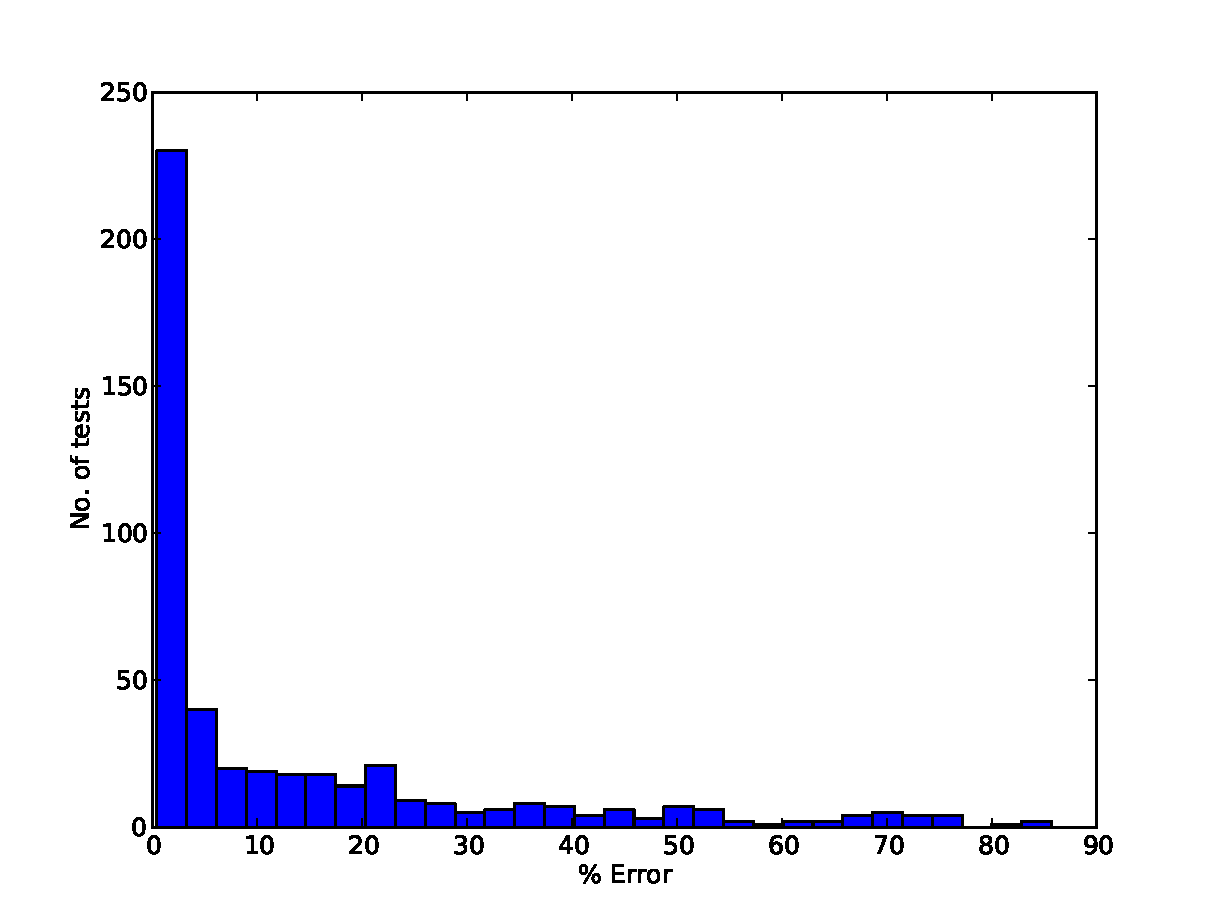
\includegraphics[width=\fullwidth]{graph/arbfitaccuracy2d.pdf}
    \scalebox{1}{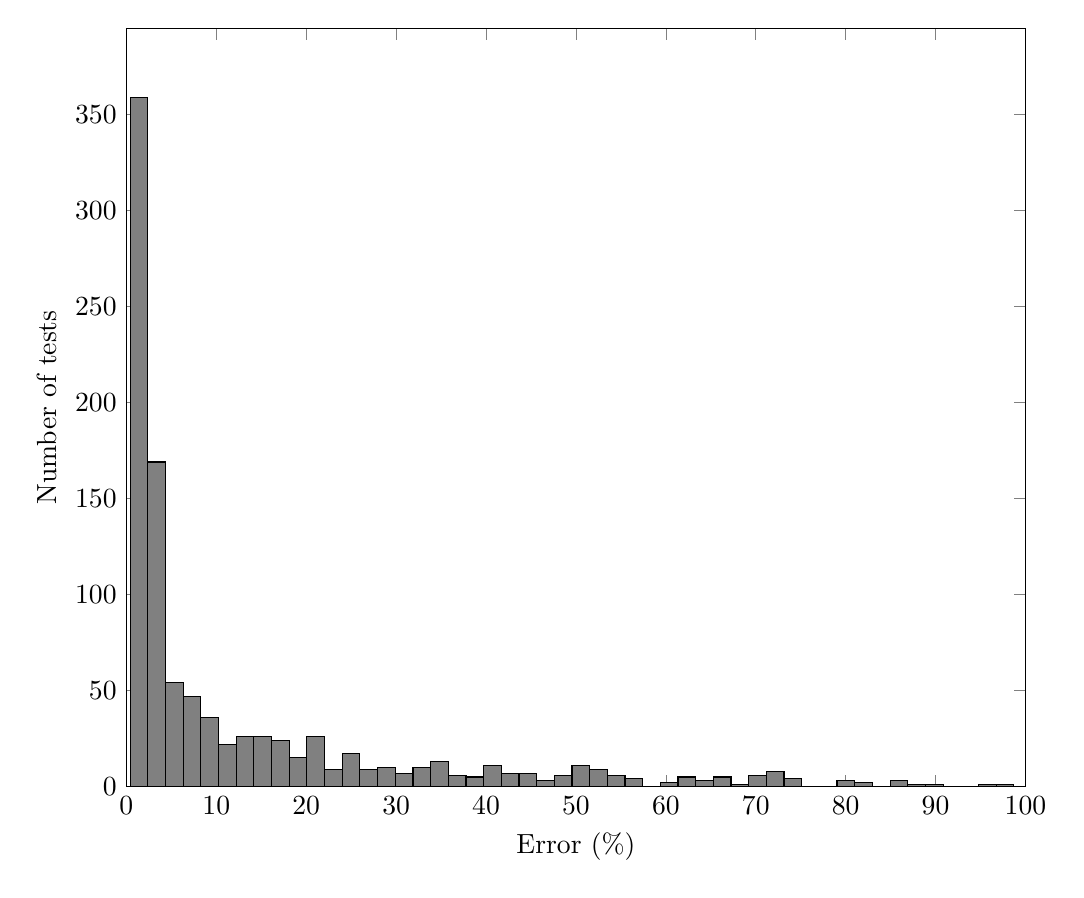
\begin{tikzpicture}
  \begin{axis}[
    width=13cm,
    ylabel=Number of tests,
    xlabel=Error (\%),
    xmin=0,xmax=100,ymin=0,]
    \addplot [ybar interval,fill=gray,draw=black] coordinates {
( 0.42510531, 359.)
( 2.39047363, 169.)
( 4.35584195,  54.)
( 6.32121027,  47.)
( 8.28657859,  36.)
(10.25194691,  22.)
(12.21731523,  26.)
(14.18268355,  26.)
(16.14805187,  24.)
(18.11342019,  15.)
(20.07878851,  26.)
(22.04415683, 9.)
(24.00952515,  17.)
(25.97489347, 9.)
(27.94026179,  10.)
(29.90563011, 7.)
(31.87099843,  10.)
(33.83636675,  13.)
(35.80173507, 6.)
(37.76710339, 5.)
(39.73247171,  11.)
(41.69784003, 7.)
(43.66320835, 7.)
(45.62857667, 3.)
(47.59394499, 6.)
(49.55931331,  11.)
(51.52468163, 9.)
(53.49004995, 6.)
(55.45541827, 4.)
(57.42078659, 0.)
(59.38615491, 2.)
(61.35152323, 5.)
(63.31689155, 3.)
(65.28225987, 5.)
(67.24762819, 1.)
(69.21299651, 6.)
(71.17836483, 8.)
(73.14373315, 4.)
(75.10910147, 0.)
(77.07446979, 0.)
(79.03983811, 3.)
(81.00520643, 2.)
(82.97057475, 0.)
(84.93594307, 3.)
(86.90131139, 1.)
(88.86667971, 1.)
(90.83204803, 0.)
(92.79741635, 0.)
(94.76278467, 1.)
(96.72815299, 1.)
(98.69352131, 0.)
    };
  \end{axis}
\end{tikzpicture}}
  \caption[Accuracy of constraint set fitting for 2 variables]{Accuracy of fitting results for a 3-constraint set into a 4-constraint set.}
  \label{fig:arbfitaccuracy2d}
\end{figure}

To increase the accuracy, a multi-start approach was taken where 25 random starting points are generated.
The largest volume set (of the 25 generated) was then used for the fitting.
Figure~\ref{fig:arbfitaccuracy2dmulti} shows the improvement in accuracy with this method.

\begin{figure}[htbp]
  \centering
%    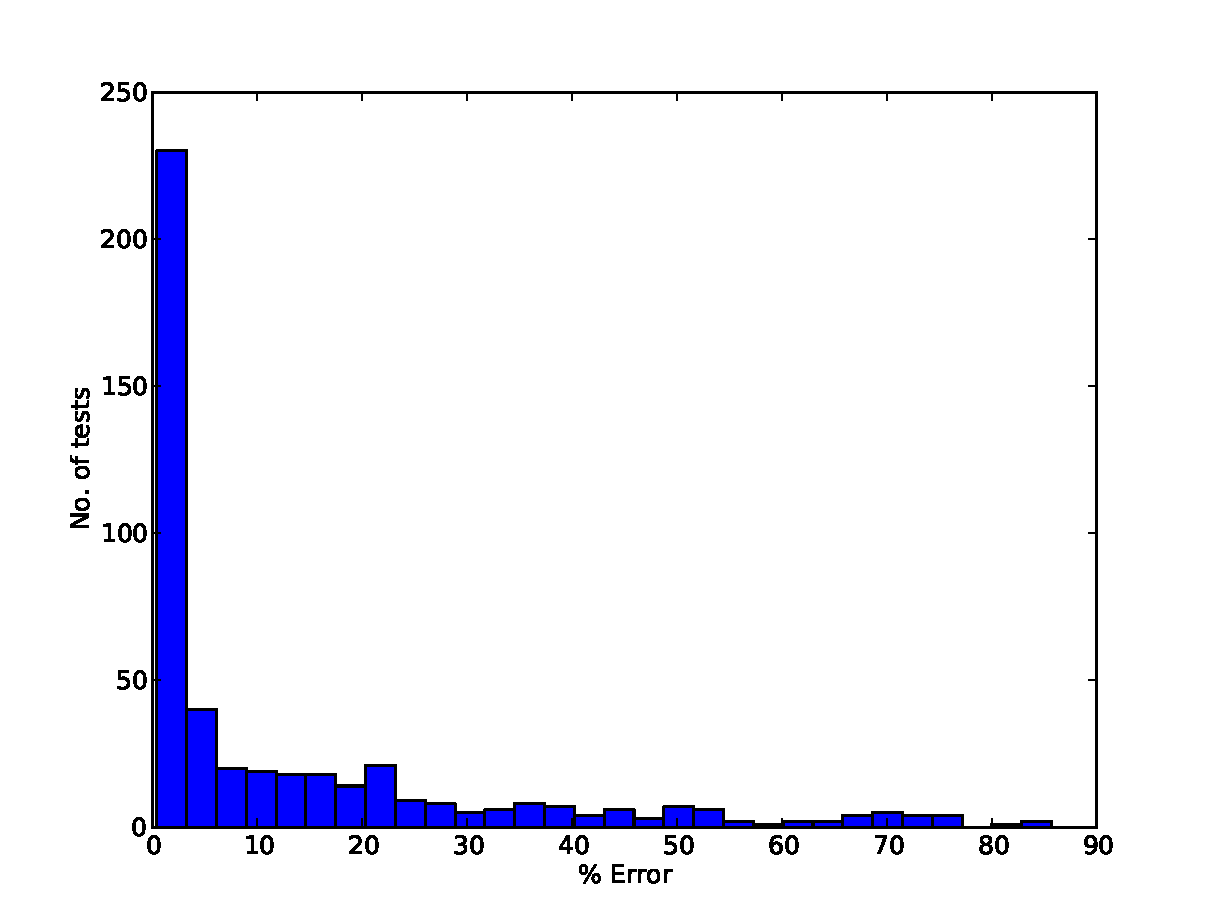
\includegraphics[width=\fullwidth]{graph/arbfitaccuracy2d.pdf}
    \scalebox{1}{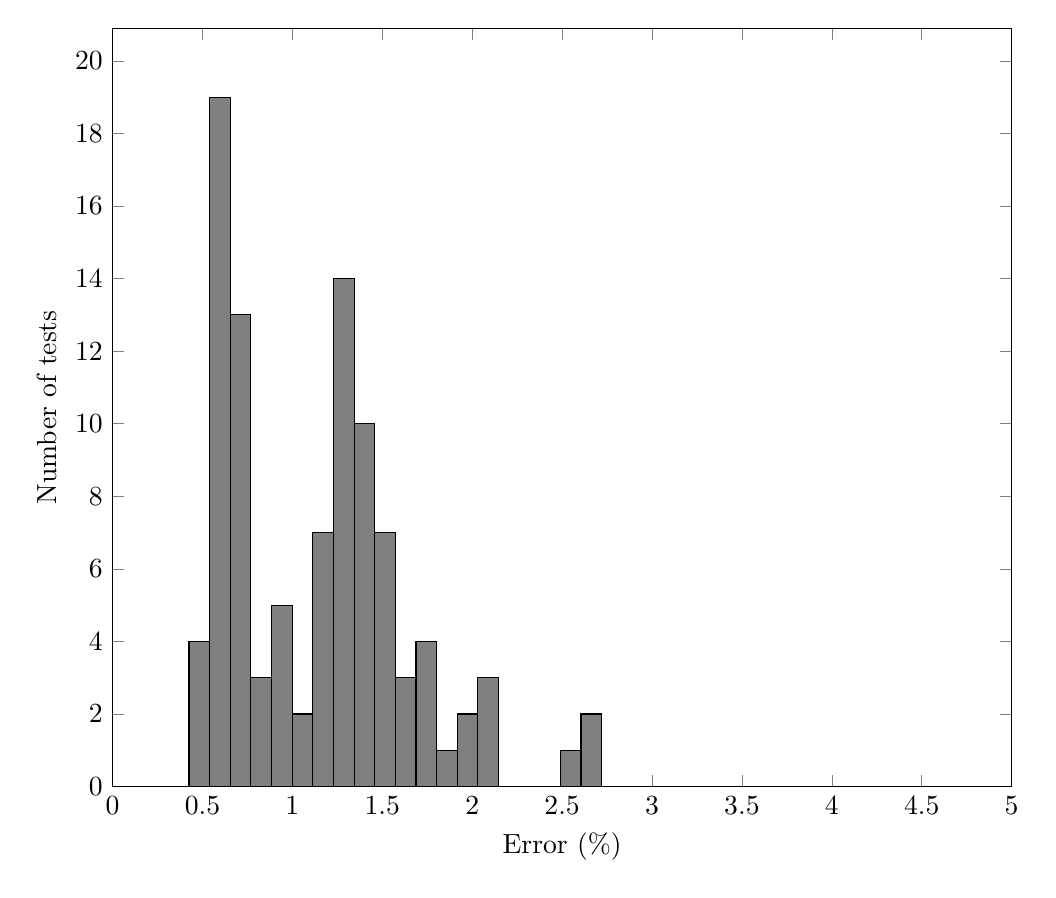
\begin{tikzpicture}
  \begin{axis}[
    width=13cm,
    ylabel=Number of tests,
    xlabel=Error (\%),
    xmin=0,xmax=5,ymin=0,]
    \addplot [ybar interval,fill=gray,draw=black] coordinates {
(0.42510531,  4.)
(0.53985223, 19.)
(0.65459915, 13.)
(0.76934608,  3.)
(0.884093,  5.)
(0.99883992,  2.)
(1.11358684,  7.)
(1.22833377, 14.)
(1.34308069, 10.)
(1.45782761,  7.)
(1.57257453,  3.)
(1.68732146,  4.)
(1.80206838,  1.)
(1.9168153, 2.)
(2.03156222,  3.)
(2.14630914,  0.)
(2.26105607,  0.)
(2.37580299,  0.)
(2.49054991,  1.)
(2.60529683,  2.)
(2.72004376,  0.)
    };
  \end{axis}
\end{tikzpicture}}
  \caption[Accuracy of constraint set fitting for 2 variables (multi-start)]{Accuracy increase from the fitting results in figure~\ref{fig:arbfitaccuracy2d} when using a multi-start approach.}
  \label{fig:arbfitaccuracy2dmulti}
\end{figure}

\subsubsection{Three variable systems}
For the three variable tests, a 4-constraint set was fitted into a 6-constraint set.
The initial constraint set was chosen to be a 3-dimensional cube -- again to allow for calculation of the optimal solution.
This test (in geometric terms) results in fitting a tetrahedron into a cube; the optimal solution being 33.33\% of the volume of the cube.
Figure~\ref{fig:arbfitaccuracy3d} shows the accuracy of this test.

\begin{figure}[htbp]
  \centering
%    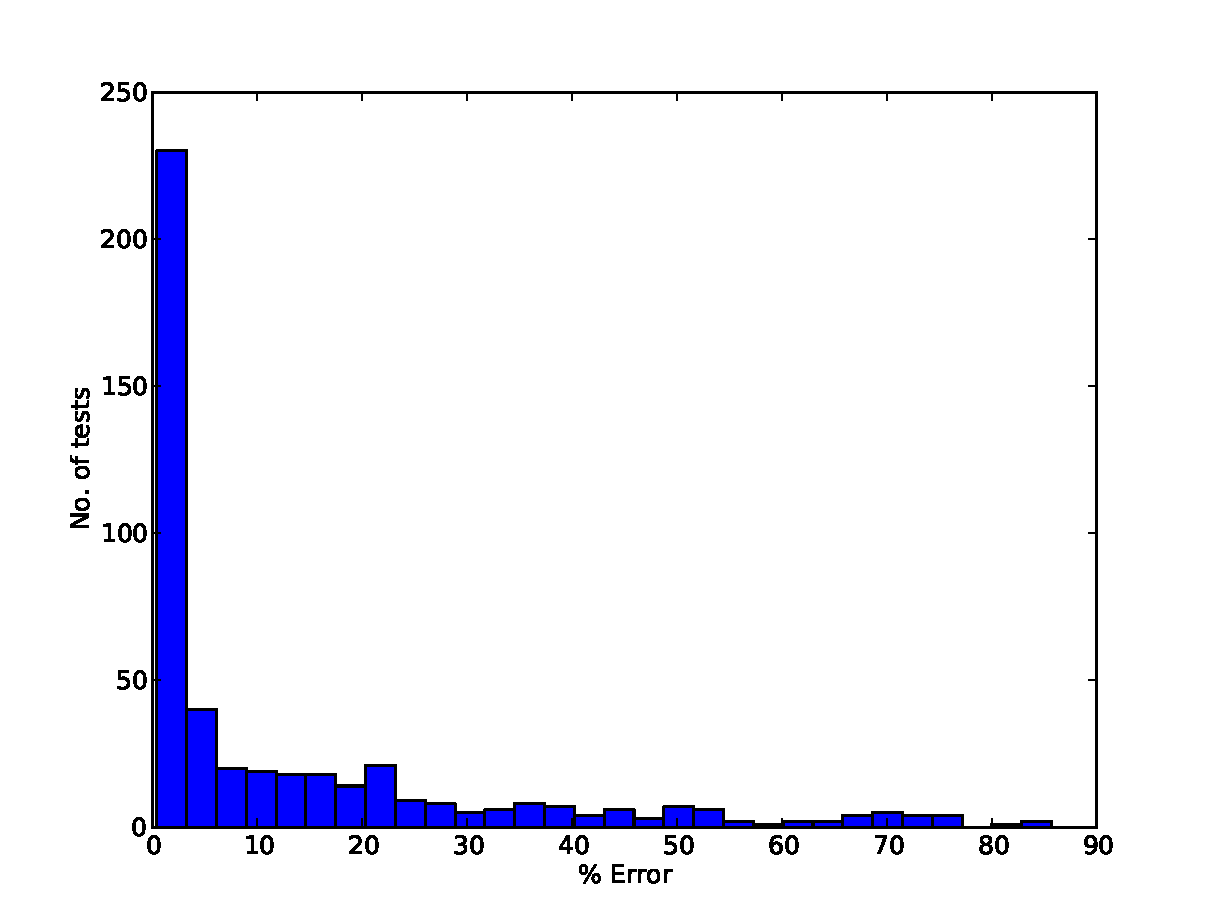
\includegraphics[width=\fullwidth]{graph/arbfitaccuracy2d.pdf}  
    \scalebox{1}{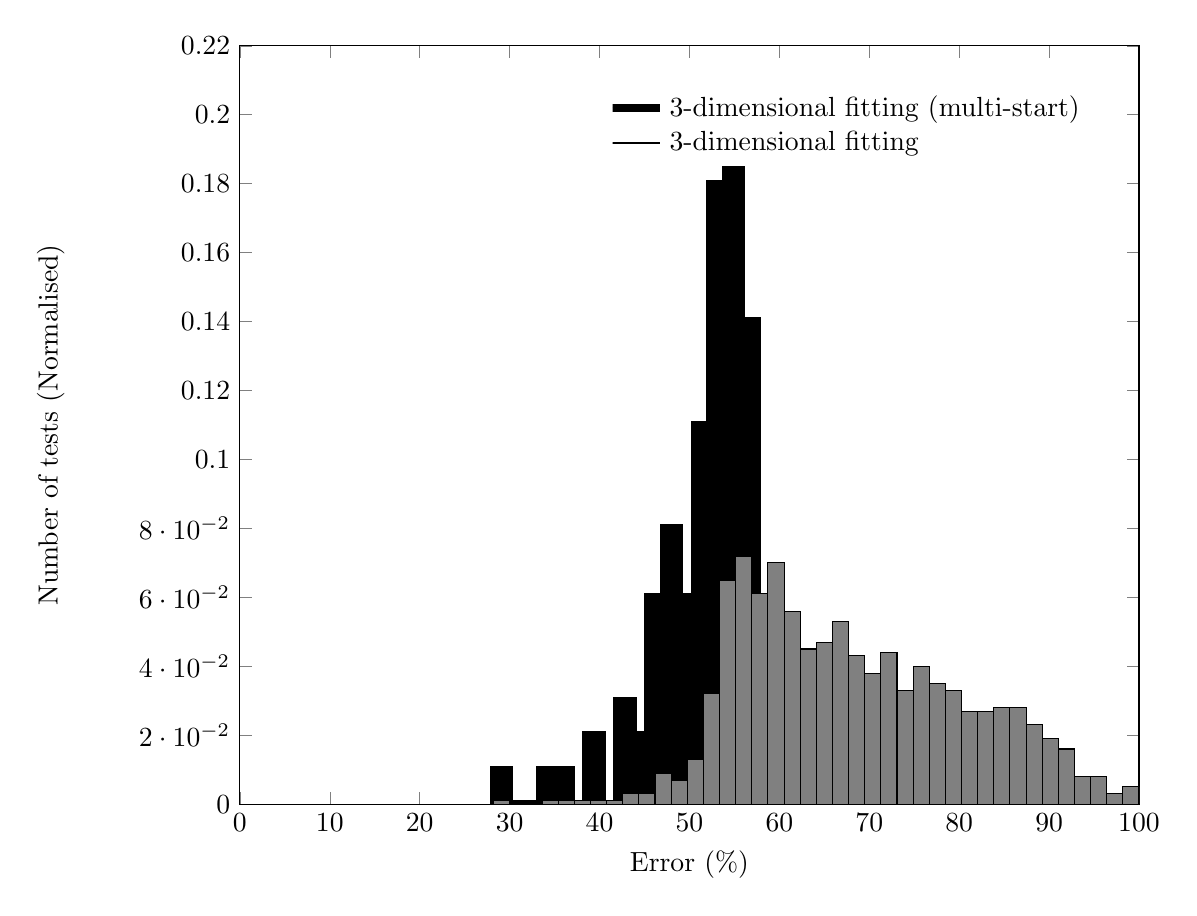
\begin{tikzpicture}
  \begin{axis}[
    width=13cm,
    ylabel=Number of tests (Normalised),
    xlabel=Error (\%),
    xmin=0,xmax=100,ymin=0,
    legend style={
      draw=none,
      at={(0.95,0.95)},
      anchor=north east,
      cells={anchor=west}}]
    \pgfplotsset{every axis y label/.append style={yshift=20pt}}


    \addplot [ybar interval,fill=black,draw=black,line width=3pt] coordinates {
 (2.82252678e+01, 1.00000000e-02)
 (2.99458083e+01, 0.00000000e+00)
 (3.16663488e+01, 0.00000000e+00)
 (3.33868893e+01, 1.00000000e-02)
 (3.51074298e+01, 1.00000000e-02)
 (3.68279703e+01, 0.00000000e+00)
 (3.85485108e+01, 2.00000000e-02)
 (4.02690513e+01, 0.00000000e+00)
 (4.19895918e+01, 3.00000000e-02)
 (4.37101323e+01, 2.00000000e-02)
 (4.54306728e+01, 6.00000000e-02)
 (4.71512133e+01, 8.00000000e-02)
 (4.88717538e+01, 6.00000000e-02)
 (5.05922943e+01, 1.10000000e-01)
 (5.23128348e+01, 1.80000000e-01)
 (5.40333753e+01, 2.00000000e-01)
 (5.57539158e+01, 1.40000000e-01)
 (5.74744563e+01, 3.00000000e-02)
 (5.91949968e+01, 2.00000000e-02)
 (6.09155373e+01, 2.00000000e-02)
 (6.26360778e+01, 0.00000000e+00)    
};

    \addplot [ybar interval,fill=gray,draw=black] coordinates {
 (2.82252678e+01, 1.00000000e-03)
 (3.00196361e+01, 0.00000000e+00)
 (3.18140044e+01, 0.00000000e+00)
 (3.36083727e+01, 1.00000000e-03)
 (3.54027410e+01, 1.00000000e-03)
 (3.71971093e+01, 1.00000000e-03)
 (3.89914776e+01, 1.00000000e-03)
 (4.07858459e+01, 1.00000000e-03)
 (4.25802142e+01, 3.00000000e-03)
 (4.43745825e+01, 3.00000000e-03)
 (4.61689508e+01, 9.00000000e-03)
 (4.79633191e+01, 7.00000000e-03)
 (4.97576874e+01, 1.30000000e-02)
 (5.15520557e+01, 3.20000000e-02)
 (5.33464240e+01, 6.50000000e-02)
 (5.51407923e+01, 7.20000000e-02)
 (5.69351606e+01, 6.10000000e-02)
 (5.87295289e+01, 7.00000000e-02)
 (6.05238971e+01, 5.60000000e-02)
 (6.23182654e+01, 4.50000000e-02)
 (6.41126337e+01, 4.70000000e-02)
 (6.59070020e+01, 5.30000000e-02)
 (6.77013703e+01, 4.30000000e-02)
 (6.94957386e+01, 3.80000000e-02)
 (7.12901069e+01, 4.40000000e-02)
 (7.30844752e+01, 3.30000000e-02)
 (7.48788435e+01, 4.00000000e-02)
 (7.66732118e+01, 3.50000000e-02)
 (7.84675801e+01, 3.30000000e-02)
 (8.02619484e+01, 2.70000000e-02)
 (8.20563167e+01, 2.70000000e-02)
 (8.38506850e+01, 2.80000000e-02)
 (8.56450533e+01, 2.80000000e-02)
 (8.74394216e+01, 2.30000000e-02)
 (8.92337899e+01, 1.90000000e-02)
 (9.10281582e+01, 1.60000000e-02)
 (9.28225265e+01, 8.00000000e-03)
 (9.46168948e+01, 8.00000000e-03)
 (9.64112631e+01, 3.00000000e-03)
 (9.82056314e+01, 5.00000000e-03)
 (9.99999996e+01, 0.00000000e+00)    
};

  \legend{3-dimensional fitting (multi-start), 3-dimensional fitting}
  \end{axis}

\end{tikzpicture}}
  \caption[Accuracy of constraint set fitting for 3 variables]{Low accuracy is obtained for higher dimensional fitting of constraint sets.}
  \label{fig:arbfitaccuracy3d}
\end{figure}

\begin{figure}[htbp]
  \centering
%    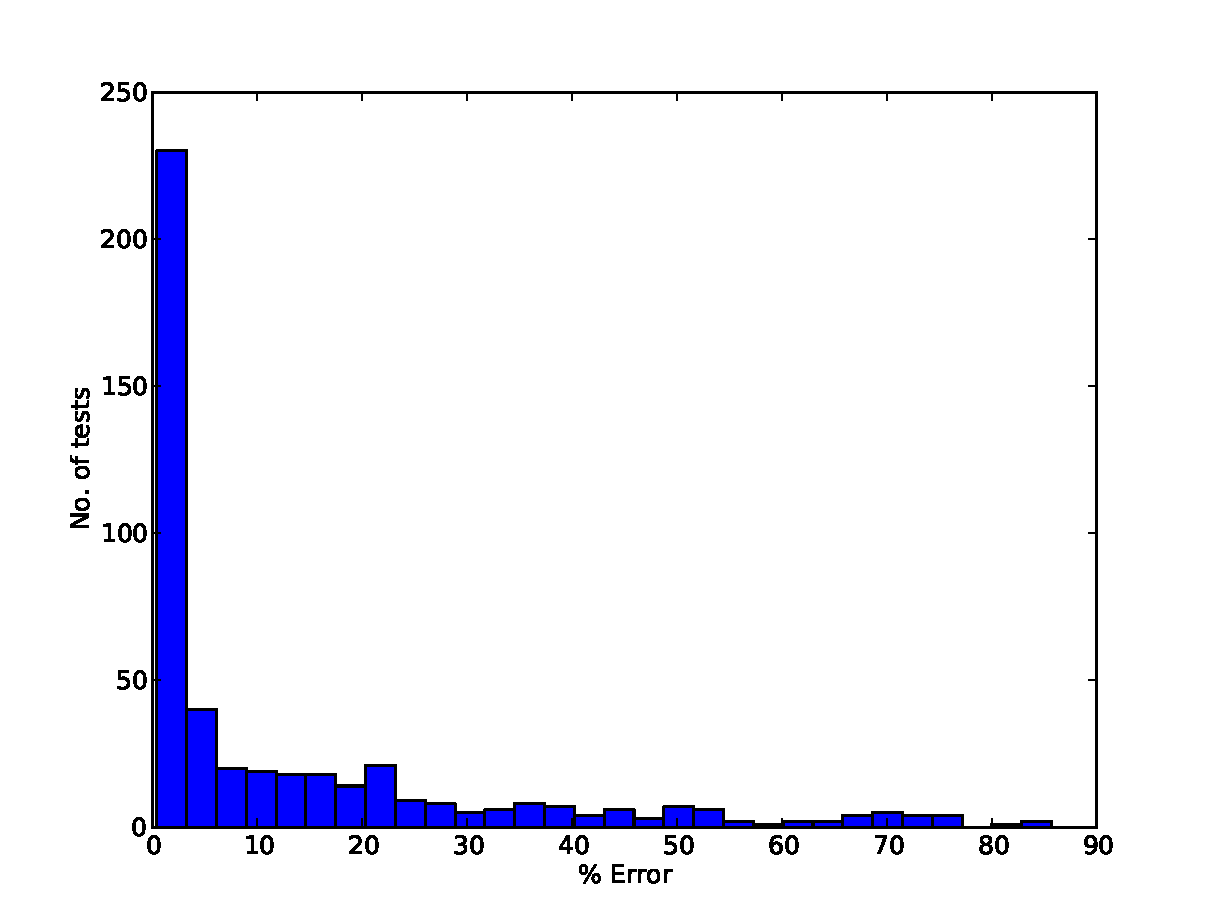
\includegraphics[width=\fullwidth]{graph/arbfitaccuracy2d.pdf}  
    \scalebox{1}{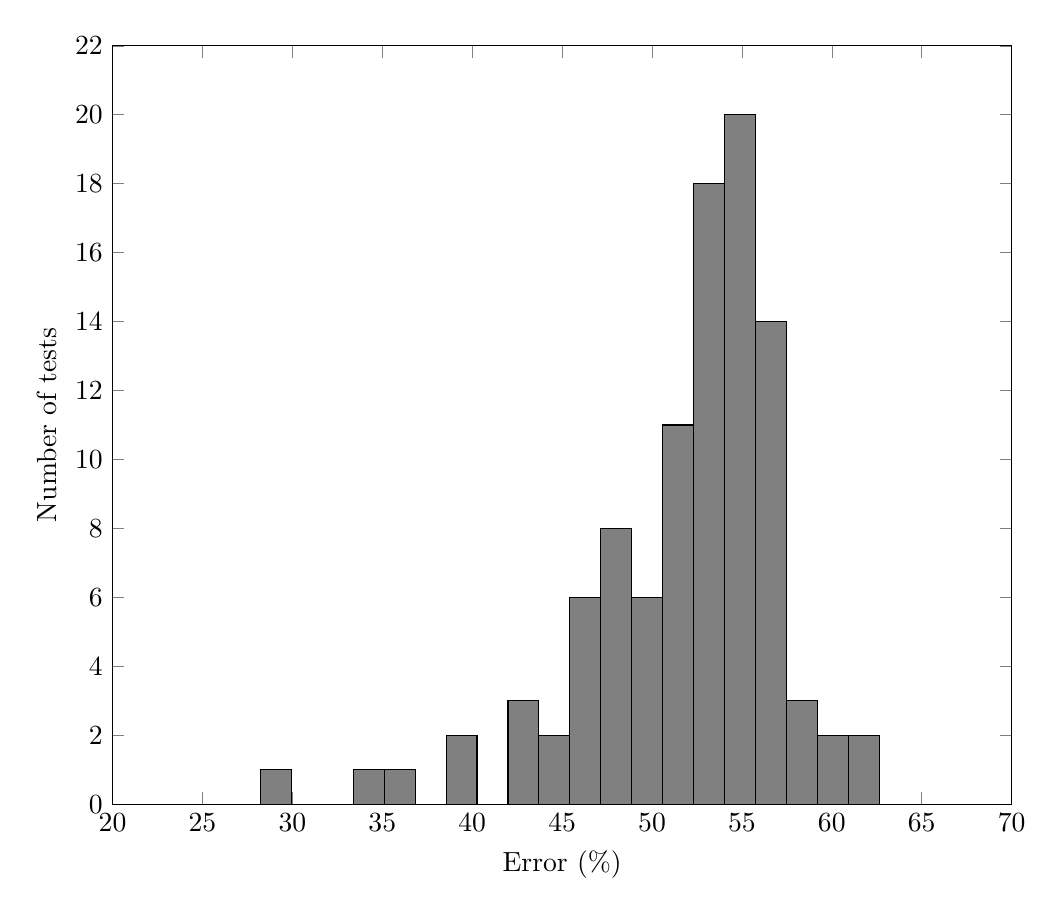
\begin{tikzpicture}
  \begin{axis}[
    width=13cm,
    ylabel=Number of tests,
    xlabel=Error (\%),
    xmin=20,xmax=70,ymin=0,]
    \addplot [ybar interval,fill=gray,draw=black] coordinates {
(28.22526783,  1.)
(29.94580833,  0.)
(31.66634883,  0.)
(33.38688933,  1.)
(35.10742983,  1.)
(36.82797033,  0.)
(38.54851083,  2.)
(40.26905133,  0.)
(41.98959183,  3.)
(43.71013233,  2.)
(45.43067283,  6.)
(47.15121333,  8.)
(48.87175383,  6.)
(50.59229433, 11.)
(52.31283483, 18.)
(54.03337533, 20.)
(55.75391583, 14.)
(57.47445633,  3.)
(59.19499683,  2.)
(60.91553733,  2.)
(62.63607783,  0.)
    };
  \end{axis}
\end{tikzpicture}}
  \caption[Accuracy of constraint set fitting for 3 variables (multi-start)]{The multi-start approach only decreases the variance of the fitting results in 3 dimensions.}
  \label{fig:arbfitaccuracy3d}
\end{figure}

None of the tests resulted in an error below 10\%.
22.8\% was the lowest error obtained from all the tests.
The low accuracy (even when using a multi-start approach) can be ascribed to the increased degrees of freedom and the ill conditioning of the problem.

\subsection{Set fitting expansion}\label{sec:setfitfuture}
The graphs shown in figure~\ref{fig:equaloifits} show a few optimal solutions obtained from the two variable tests of section~\ref{sec:2dfitting}.
It can be seen that even though the sets are not equal, the output Operability Index \citep{vinsonphd} calculated for all of them are equal.
\begin{figure}[htbp]
  \centering
%    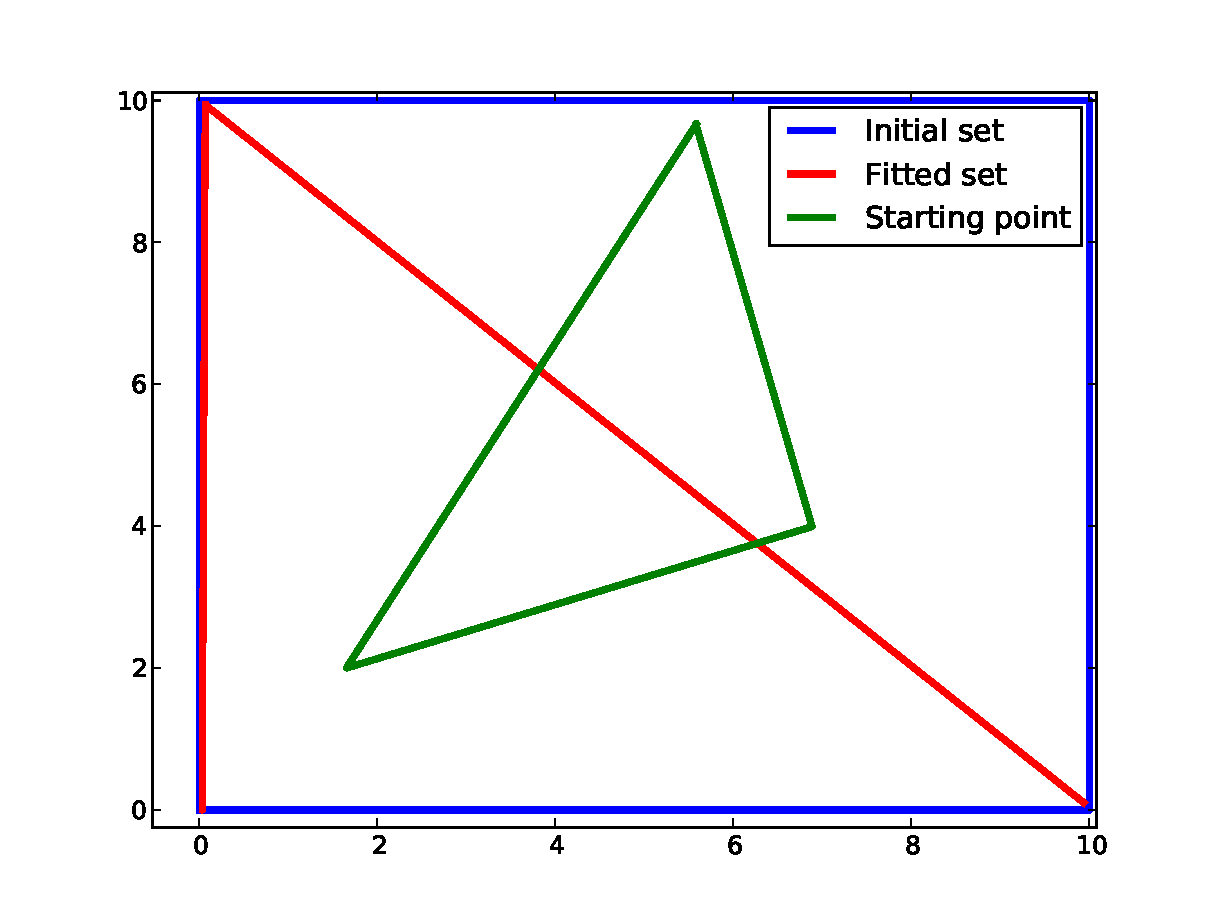
\includegraphics[width=7.8cm]{graph/2dfit1.pdf}
    \scalebox{1}{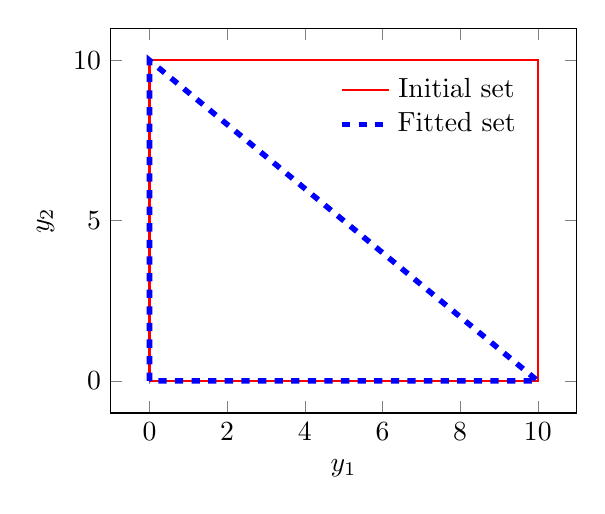
\begin{tikzpicture}
  \begin{axis}[
    width=7.5cm,
    xlabel=$y_1$,
    ylabel=$y_2$,
    legend style={
      draw=none,
      fill=none,
      at={(0.9,0.9)},
      anchor=north east}]
    %AOS
    \addplot[color=red,thick] coordinates {
      (0,0)
      (0,10)
      (10,10)
      (10,0)
      (0,0)
    };
    %Fit
    \addplot[color=blue,line width=2pt, dashed] coordinates {
      (0,0)
      (0,10)
      (10,0)
      (0,0)
    };
    \legend{Initial set, Fitted set}
  \end{axis}
\end{tikzpicture}
}
    %\qquad
%    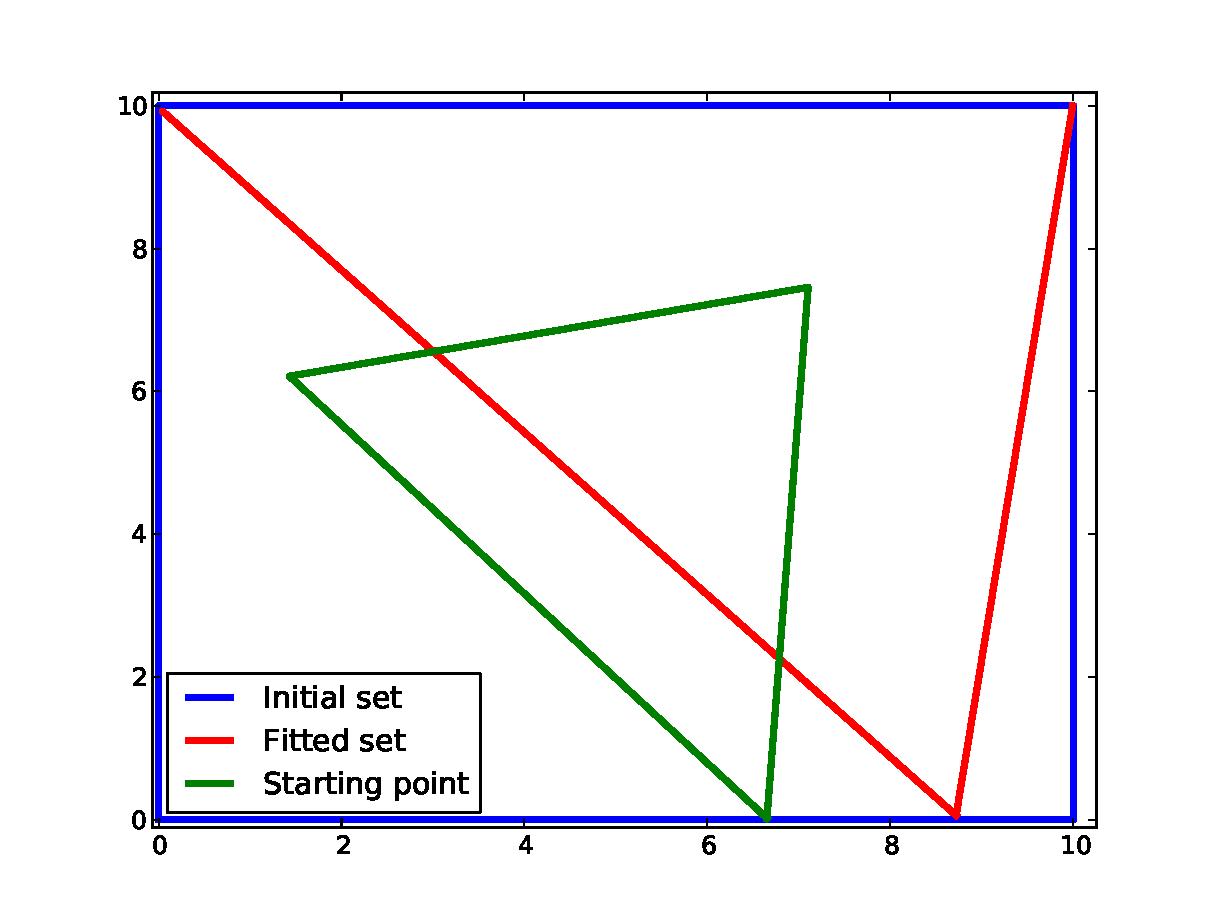
\includegraphics[width=7.8cm]{graph/2dfit2.pdf}
    \scalebox{1}{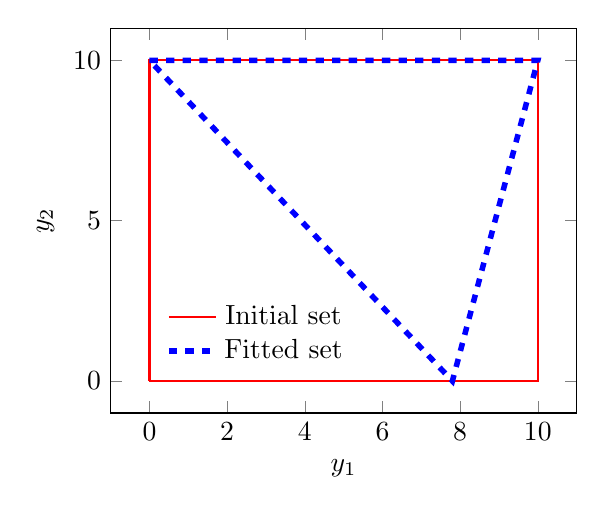
\begin{tikzpicture}
  \begin{axis}[
    width=7.5cm,
    xlabel=$y_1$,
    ylabel=$y_2$,
    legend style={
      draw=none,
      fill=none,
      at={(0.1,0.1)},
      anchor=south west}]
    %AOS
    \addplot[color=red,thick] coordinates {
      (0,0)
      (0,10)
      (10,10)
      (10,0)
      (0,0)
    };
    %Fit
    \addplot[color=blue,line width=2pt, dashed] coordinates {
      (0,10)
      (10,10)
      (7.8,0)
      (0,10)
    };
    \legend{Initial set, Fitted set}
  \end{axis}
\end{tikzpicture}
}
  \caption[Equal size constraint set fits]{Different sets fitted with an equal size and equal calculated Operability Index.}
  \label{fig:equaloifits}
\end{figure}

From these results the following observations regarding the Operability Index of \citet{vinsonphd} can be made:
\begin{itemize}
\item the Operability Index is a measure of moveability and emphasises the need for inputs to have a good working range to achieve outputs.
\item all of the input and output space are of equal importance in the Operability Index.
\end{itemize}

It is intuitive that certain sections of the input or output space are of greater importance when considering process economics, sensitivities, etc..
It would therefore be a sensible approach to take into consideration an additional objective function when fitting constraint sets (or when making any changes to the input or output spaces).
Fitting a set as the volume integral of the following possible objective functions would be favourable:
\begin{itemize}
\item Economic objective functions would generate an operating region that maximises profit or minimises cost.
\item Sensitivity functions would identify regions that are problematic to control in and favour them less.
\item Design cost functions would aid in process design when processes are being designed or modified -- costs can be directly related to the improvement in control.
\end{itemize}
These improvements to the constraint set fitting are suggested as a topic for future research.

% Local Variables:
% TeX-master: "AHC_thesis"
% End: